\documentclass[ASNA,twocolumn]{USG} %twocolumn
\usepackage{anyfontsize} %

\usepackage{colortbl}   % For coloring table lines
\usepackage{xcolor}     % For color definitions
\usepackage{graphicx}
\usepackage[utf8]{inputenc}
\usepackage[misc,geometry]{ifsym} 
\usepackage{fontspec}
\usepackage{fontawesome}
\usepackage{academicons}
\usepackage{color}
\usepackage{hyperref} 
\usepackage{aas_macros}
\usepackage[bottom]{footmisc}
\usepackage{supertabular}
\usepackage{afterpage}
\usepackage{url}
\usepackage{pifont}
\usepackage{multicol}
\usepackage{multirow}
\usepackage{algorithm}
\usepackage{algpseudocode}

% Configuration begins for listing -----------------------------------------------------------------
\usepackage{listings}
\usepackage{colortbl}
\usepackage{fancyvrb}
\fvset{frame=double,framesep=2mm,fontfamily=courier,
	fontsize=\scriptsize,
	framerule=.3mm,
	numbersep=1mm,
	commandchars=\\\{\}}

\lstdefinelanguage{IT} {
	morekeywords={Program, Task, Function, Type},
	morekeywords={[2]Define, Initialize, Environment, Stages, Computation, Partition, Compute},
	morekeywords={[3]new, if, else, do, for, in, step, sequence, at, while, and, or, foreach, from, of, current},
	morekeywords={[4]Repeat, Where, Epoch, Activate},
	morekeywords={[5]divides, partitions, Sub, sub, partitioned, un, ordered, unordered, partition, replicated},
	morekeywords={[6]Space, A, B, C, D, E, F, G, H, I, J, K, L, M, N, O, P, Q, R, S, T, U, V, W, X, Y, Z},
	morekeywords={[7]link, link_or_create, create},
	morekeywords={[8]name, task, environment, partition, initialize},
	morekeywords={[9]@Extern, @Language, @Libraries, @Includes},
	morekeywords={[10]Kernel},
	sensitive=true,
	morecomment=[l]{//},
	morestring=[b]''
}

\lstdefinelanguage{intermIT} {
	morekeywords={Flow_Initialization, Flow_Stage},
	morekeywords={[2]Space},
	morekeywords={[3]R, W, move, to, comm, root},
	sensitive=true,
	morecomment=[l]{//}
}

\lstdefinelanguage{mappingIT} {
	morekeywords={mapping, task, model, lps, id, pps, no},
	morekeywords={[2]Space, Model, Root},
	morekeywords={[3]A, B, C, D, E, F, Z},
	sensitive=true,
	morecomment=[l]{//}
}

\lstnewenvironment{codeExampleListing}[2] {
	\lstset{language=IT,                basicstyle={\footnotesize\singlespacing},            keywordstyle={\footnotesize\itshape\color[rgb]{0.1,0.1,0.9}},
		keywordstyle=[2]{\footnotesize\itshape\color[rgb]{0.9,0.1,0.1}},
		keywordstyle=[3]{\itshape},
		keywordstyle=[4]{\bf\itshape\color[rgb]{0.2,0.5,0.9}},
		keywordstyle=[5]{\itshape},
		keywordstyle=[6]{\ttfamily\bfseries\color[rgb]{0.0,0.2,0.9}},
		keywordstyle=[7]{\itshape},
		keywordstyle=[8]{\itshape},
		keywordstyle=[9]{\ttfamily\bfseries\color[rgb]{0.5,0.2,0.9}},
		keywordstyle=[10]{\scriptsize\itshape\color[rgb]{0.1,0.1,0.9}},
		numbers=left,
		tabsize=2,
		numbersep=1pt,
		basewidth=0.48em,
		commentstyle=\color[rgb]{0.1,0.4,0.1},
		captionpos=b,
		label=#1, caption=#2
	}
}{}

\lstnewenvironment{explanationListing}[3] {
	\lstset{language=IT,
		tabsize=4,
		basicstyle={#3\singlespacing},
		keywordstyle={\itshape\color[rgb]{0.1,0.1,0.9}},
		keywordstyle=[2]{\itshape\color[rgb]{0.9,0.1,0.1}},
		keywordstyle=[3]{\itshape},
		keywordstyle=[4]{\bf\itshape\color[rgb]{0.2,0.5,0.9}},
		keywordstyle=[5]{\itshape},
		keywordstyle=[6]{\ttfamily\bfseries},
		keywordstyle=[7]{\itshape},
		keywordstyle=[8]{\itshape},
		keywordstyle=[9]{\ttfamily\bfseries\color[rgb]{0.5,0.2,0.9}},
		keywordstyle=[10]{\itshape\color[rgb]{0.1,0.1,0.9}},
		numbers=none,
		numbersep=1pt,
		basewidth=0.48em,
		commentstyle=\color[rgb]{0.1,0.4,0.1},
		captionpos=b,
		label=#1, caption=#2
	}
}{}  

\lstnewenvironment{mappingListing}[2] {
	\lstset{language=mappingIT,
		basicstyle={\footnotesize\singlespacing},
		keywordstyle={\itshape\color[rgb]{0.1,0.1,0.9}},
		keywordstyle=[2]{\itshape\color[rgb]{0.9,0.1,0.1}},
		keywordstyle=[3]{\itshape},
		numbers=none,
		tabsize=4,
		basewidth=0.48em,
		commentstyle=\color[rgb]{0.1,0.4,0.1},
		captionpos=b,
		label=#1, caption=#2
	}
}{}

\lstnewenvironment{interimC}[2] {
	\lstset{language=C,
		basicstyle={\footnotesize\singlespacing},
		keywordstyle={\itshape\color[rgb]{0.1,0.1,0.9}},
		numbers=left,
		numbersep=1pt,
		tabsize=2,
		basewidth=0.48em,
		commentstyle=\color[rgb]{0.1,0.4,0.1},
		captionpos=b,
		label=#1, caption=#2
	}
}{}

% Configuration ends for listing ------------------------------------------------------------------


\usepackage{steinmetz}
\graphicspath{{./images/}}
%\specialissue{Morphologic Hard and Soft Tissue Changes following Tooth
%Extraction in Different Maxilla and Mandible Anatomic Areas: Current
%Knowledge, Prognostic Factors Analysis, and Clinical Management}

\articletype{ORIGINAL ARTICLE}%
\subarticletype{High-performance Computing}

%\received{20 January 2023}
%\revised{21 January 2023}
%\accepted{22 January 2023}
\journal{Concurrency and Computation: Practice and Experience}
%\volume{0}
%\copyyear{2026}
\startpage{1}
%\articledoi{10.1002/0000}

%\raggedbottom

%%
%\renewcommand\ShowFrameLinethickness{0.15pt}
%\renewcommand*\ShowFrameColor{\color{red}}


\begin{document}
\title{HighP5 Compiler for Hierarchical Distributed Memory Machines}
%\subtitle{Subtitle}
\transtitle{HighP5 Compiler for Hierarchical Distributed Memory Machines}
%\subtranstitle{trans-subtitle}
\author[1]{Muhammad Nur Yanhaona}[https://orcid.org/0000-0003-2450-3377][\linkedin{https://bd.linkedin.com/in/yanhaona}]
\author[2]{Andrew Grimshaw}[https://orcid.org/0000-0002-2072-9873]

\authormark{yanhaona \textsc{et al.}}
\titlemark{HighP5 Compiler for Hierarchical Distributed Memory Machines}

\address[1]{\orgdiv{Computer Science and Engineering Department, }\orgname{BRAC University, }%
\orgaddress{\state{Dhaka, }\country{Bangladesh}}}

\address[2]{\orgdiv{Department of Computer Science, }\orgname{University of Virginia, }%
\orgaddress{\state{Virginia, }\country{United States}}}

\corres{Muhammad Nur Yanhaona  (\email{nur.yanhaona@bracu.ac.bd}) ~|~ Andrew Grimshaw (\email{grimshaw@virginia.edu})}

%\editor{\textbf{Academic Editor:} Alex ~|~ \textbf{Guest Editor:} Andrew A. Rooney}

\presentaddress{Kha 224 Pragati Sarani, Merul Badda, Dhaka 1212, Bangladesh}

\fundingInfo{This work is partially funded by the XSEDE: Extreme Science and Engineering Discovery Environment project of National Science Foundation, USA. The fund was granted to Andrew Grimshaw for his investigation on GFFS: a Global Federated File System that connects compute and storage resources across university campuses and supercomputing centers for fostering research collaboration.}

\keywords{Parallel Programming | High-performance Computing | Automatic Synchronization | Communication Optimization | Compiler | MPI | Pthreads}

\transkeywords{Parallel Programming | High-performance Computing | Automatic Synchronization | Communication Optimization | Compiler | MPI | Pthreads}

\abstract[ABSTRACT]{The landscape of high performance parallel computing is currently dominated by distributed, hierarchical machines. Supercomputers and computer clusters now connect multicore processors with local memories through high-speed networks where both the former and the latter are themselves hierarchical in nature due to multi-level caches in NUMA-nodes and complex inter-connection topologies among server racks and cabinets. Careful data and computation placement, low-overhead shared-data synchronization within cores of a node, and optimized communication across nodes over the network are critical for good program performance in present-day machines. For HighP5 programming language, all these aspects are challenging compilation issues as HighP5 is a declarative programming language where programmers write a pseudocode-like parallel program where only intensions regarding these aspects are specified and their proper implementation is left for the compiler to determine. This article discusses how the HighP5 compiler solves the issues related to efficient memory-management, intra-node synchronization, and communication in hierarchical distributed machines and compares performance of HighP5 executables for some building block reference problems against optimized hand-written MPI codes. Although the design decisions and algorithmic elements discussed in this writing are part of the HighP5 compiler; they are generic enough to apply to any parallel programming language that works in distributed, hierarchical machines and wants to abstract away data synchronization and communication operations from the programmers.}

 \transabstract[transABSTRACT]{The landscape of high performance parallel computing is currently dominated by distributed, hierarchical machines. Supercomputers and computer clusters now connect multicore processors with local memories through high-speed networks where both the former and the latter are themselves hierarchical in nature due to multi-level caches in NUMA-nodes and complex inter-connection topologies among server racks and cabinets. Careful data and computation placement, low-overhead shared-data synchronization within cores of a node, and optimized communication across nodes over the network are critical for good program performance in present-day machines. For HighP5 programming language, all these aspects are challenging compilation issues as HighP5 is a declarative programming language where programmers write a pseudocode-like parallel program where only intensions regarding these aspects are specified and their proper implementation is left for the compiler to determine. This article discusses how the HighP5 compiler solves the issues related to efficient memory-management, intra-node synchronization, and communication in hierarchical distributed machines and compares performance of HighP5 executables for some building block reference problems against optimized hand-written MPI codes. Although the design decisions and algorithmic elements discussed in this writing are part of the HighP5 compiler; they are generic enough to apply to any parallel programming language that works in distributed, hierarchical machines and wants to abstract away data synchronization and communication operations from the programmers.}

%\abbr{5-FU, 5-fluorouracil; CFD, computational fluid dynamics; CH, channel; EFS, event-free survival; GBM, glioblastoma multiforme; OS, overall survival; PFS, progression-free
%survival; SD, standard deviation.}

%\contributed{Hao Zhang and Pengyue D. Guo contributed equally to this study.}

%\dedicated{Dedicated to Srivivasa Ramanujano on the occasion of his 125th birth anniversary.}

%\copyright{This is an open access article under the terms of the \href{Creative Commons Attribution-NonCommercial}{Creative Commons Attribution-NonCommercial} License, which permits use, distribution and reproduction in any medium, provided the
%original~work~is~properly cited and is not used for commercial purposes.
%\\[5pt]
%  ©  2024 The Author(s) \textit{AIChE Journal} published by Wiley Periodicals LLC on behalf of American Institute of Chemical Engineers.}

%\openaccessstatement

\maketitle
%\afterpage{\aftergroup\restoregeometry}

%\onecolumn

\section{Introduction}
\label{sec:introduction}
The abundance of distributed memory machines in high performance computing is evident from the TOP500 \citep{Dongarra2011} supercomputers list. For several decades running, all the machines in the list are distributed memory machines. In early days, these machines were pure distributed memory machines: connecting unicore CPUs via some high speed networks. However, now almost all supercomputers have multicore CPUs and GPUs interconnected through complex interconnection networks. For example, the first exascale machine Frontier \citep{10485138} has one 64-core AMD CPU and 4 integrated GPUs as building block nodes. Consequently, these machines can be called distributed shared-memory multicomputers where parts of the total aggregate distributed memory of the machines are shared among groups of processing units. The same characterization holds for compute clusters prevalent in campuses and organizations, as they comprise commodity machines armed with multicore CPUs and GPUs. This march of distributed shared-memory multicomputers -- henceforth, we will call them just distributed memory machines for simplicity -- should continue without some tectonic shift in the architecture of sillicon-based computers due to the inherent scalability problem with hardware cache-coherency protocol \citep{10.1145/158439.158907} for large purely shared-memory computers.

The big question is how to utilize distributed memory machines in high performance computing effectively. Although the extent of exa-scale and peta-scale machines' may marvel an onlooker, actually the available computation power historically always lags behind application demand \citep{Snyder:1986:TAS:17814.17826}. The reason is that algorithms for most interesting problems are of quadratic or higher order, while improvement in computation capacity is linear; and larger capacities always drive application interest towards even larger input and higher precision \citep{10.1145/42411.42415}. Since performance is the supreme concern, making the best use of the capacities of underlying execution platform is essential. However, exploiting the capacities does not come from just a better parallel algorithms, it requires balancing communication with computation, optimizing data synchronization, and better distribution of computation and data \citep{Foster:1995:DBP:527029} -- all of which are platform dependent. Consequently, it is fair to say that high performance parallel computing is hard except for some simple cases. 

The desire to eke out all features of a target execution platform led to the dominance of low-level primitives or language extensions, such as, MPI \citep{Walker96mpi:a}, Pthreads \citep{10.5555/263953}, and CUDA \citep{Nickolls:2008:SPP:1365490.1365500} in parallel computing for several decades. However, effective utilization of recent distributed memory machines require combining these primitives that are individually difficult. Furthermore, although the best performance is attainable using these primitives, the primitives themselves do not inherently promote good decision making about a program implementation; rather, programmers' ad hoc understanding of the machine architecture is the key. For example, it is shown that incorporating network topology-dependent reasoning significantly improves MPI program implementations' performance \citep{10.1145/2488551.2488564}. However, with the complexity of both interconnection network and node architecture on the rise, such ad hoc decision making has also become increasingly difficult.

Due to this increasing difficulty of parallel programming in newer machines, the interest of high-level programming languages that abstract away some aspects of data distribution, synchronization, and communication has grown. The approaches in this regard widely varies, from {\textit{pragma} pre-processor parallization directives in OpenACC \citep{farber2016parallel} for accelerator-like platforms, multi-paradigm parallel library integrations in Julia \citep{lin2021comparing} for different architectures, detailed data distribution and computation placement facilities in KoKKOS \citep{trott2021kokkos}, or a simpler cleaner uniform partitioned shared-memory programming in PGAS languages \citep{Yelick:2007:PPU:1278177.1278183}. 
	
    
HighP5 \citep{yanhaona2024highp5} is unique among the new language and library alternatives to low-level coding in the sense that it allows programmers to map computation and data to arbitrary partition levels of a hierarchical distributed memory machine. HighP5 is a declarative programming language where programmers express the flow of computations using a pseudocode-like description and specify a hierarchical data distribution that computations manipulate. They then explicitly `map' the computations and data to different levels of hierarchy of the target execution platform. The compiler does the necessary index transformation, synchronization insertion, and data communication that are needed for the correct behavior and good performance of the executable code. This breakdown of responsibilities enables efficient executable generation of the same source program for different target platforms using different mapping configurations.  
	
This article discusses the working principle of the HighP5 compiler for distributed memory platforms with a particular emphasis on data part representation, logic, and algorithms for automatic data synchronization and communication. Two critical concerns in this regard are to minimize the cost of decision making code that compiler inserts in-between users' application logic so that performance debugging is easy and to optimize the implementation of data synchronization and communication logic. The compiler generates MPI+Pthreads hybrid code where synchronization within a shared-memory region is achieved using Pthreads semaphores and barriers and various forms of MPI point-to-point and group communications are employed for syncing data among distributed memory parts. Careful attention is paid to the use of appropriate MPI collective communication primitives whenever possible to take the advantage of separate collective communication networks that are common on modern supercomputers \citep{10.1145/1088149.1088183} and HPC environments \citep{6490322}\citep{10.1145/329366.301116}. Furthermore, the compiler applies asynchronous communication and code reordering to maximize computation-communication overlap. 
	
The article also analyzes the performance of HighP5 executables for three building block problems from dense and sparse linear algebra, and finite-value method in comparison to optimized handwritten benchmark code implemented in plain MPI on the Fugaku supercomputer \citep{sato2021co}. The comparative analysis exposes some important implementation aspects of automatic synchronization and communication that greatly impact the performance at scale.
	
The contribution of this article is important mainly from two respects. First, the techniques and algorithms HighP5 distributed memory compiler uses are not specific to the language. Rather, it treats efficient data-parts representation and communication requirement calculation in a hierarchically partitioned distributed memory machine as generic problems whose solutions should be useful to current and future language compilers that target similar machine architectures. Second, although the literature on languages, platform improvements, and performance assessments is rich in parallel computing; there is a dearth of publications on compilers that this article amplifies.  
	
\section{Related Work}
\label{sec:related-work}
The extent of compilers' responsibilities in parallelizing high performance computing programs evolved with the evolution of the parallel hardware architectures. We can track early efforts on automatic extraction of fine-grained parallelism from functional languages programs in languages like SISAL \citep{osti_10192282}\citep{FEO1990349} and VAL \citep{10.1145/357153.357157}. Parallel hardware researchers at that time were focused on building data flow machines \citep{GURD198549}\citep{10.1145/27633.28055} that can utilize fine-grained parallelism effectively. However, with the lack of success with data-flow machine architectures, interest in fine-grained parallelism extraction also died.
	
Early successful supercomputers are shared-memory machines that connect a large number of independent processing units to a shared memory \citep{10.5555/1623264.1623335} \citep{10.1145/1480083.1480098} \citep{hord1982illiac}. Their success ushered great interest in shared-memory parallel programming, in particular, in parallelizing compilers \citep{10.1145/234313.234417}\citep{10.1145/193209.193217}. A parallelizing compiler takes a sequential code, does data flow analyses of the code to identify operations that can be done in parallel, then generates an equivalent parallel program by segregating parallel parts and inserting synchronization operations in appropriate places. However, the scalability problem with concurrent memory accesses from a large number of processors and the difficulty of implementing hardware cache coherence protocol in large machines led to the demise of shared memory machines in high performance computing.
	
The advent of early distributed memory machines practically bode farewell to parallelizing compilers ~\citep{10.1145/1238844.1238851}. The reason behind is the gross disparity between the cost of a communication and the cost of a computation, with former being hundred to thousand times higher than the latter. Foster's influential methodology of parallel programming \citep{Foster:1995:DBP:527029} is a good mechanism to formally explore the underlying problem. According to Foster, effecient parallel programming in a distributed memory machine requires: first, a parallel algorithm; second, determining communication among parallel parts; third, agglomerating the parts into larger units to reduce communications; and forth, mapping those units to the parallel processors of the target execution platform. Parallelizing compilers were good at the first two tasks. However, generic solution to agglomeration and mapping is a computationally hard problem, thus, unsolvable for compilers.  
	
A key takeaway from that era of high performance computing is that programmers should specify appropriate data distribution and implicitly/explicitly delineate the positions of the code where data synchronization among overlapping data parts located in different places of a distributed memory machine. The compilers should implement the communication and synchronization logic based on programmers' direction. Co-array FORTRAN \citep{10.1145/289918.289920}, HPF \citep{219857} \citep{MEHROTRA1998325}, C** \citep{10.1007/3-540-57502-2_56}, and NESL \citep{10.5555/865114} are examples of languages, among many others, built with this vision at that time. However, the programming model that eventually dominated is the Message Passing Standard (MPI) \citep{10.1007/978-3-0348-8534-8_21}, which is a realization of Hoare's Communicating Sequential Processes (CSP) \citep{10.1145/359576.359585}. MPI is a low-level library programming with C and FORTRAN bindings, where programmers control all aspects of computation and communication, and hardware engineers focus on efficient implementation of different MPI communication primitives. This role breakdown practically relieves the language compiler from all responsibilities related to parallelism. 
	
There are many arguments for MPI's predominance in high performance computing. Giving programmers the utmost control on all aspects of parallel programming undoubtedly promotes the best performance, which is the prime concern, and argued as the main contributor's to MPI's success. However, optimized MPI programs are difficult to write and equally difficult to debug. The key problem with the MPI programming is that there is no clean abstraction available to the programmers to reason about the capabilities of the execution platform. Consequently, ad-hoc optimizations are needed in the code to make the best use of the hardware. Furthermore, a plethora of explicit communication codes hide the algorithmic logic of the implementation.
	
MPI is still prominent in this era of exascale computing \citep{https://doi.org/10.1002/cpe.4851}. However, the advent of multicore processors and GPUs in the beginning of this millennium inspires a renewed interest in high-level parallel language alternatives to MPI programming. Supercomputers are built now a days using multicore CPUs and GPUs as nodes connected via one or more high-speed hierarchical interconnection networks. There are regions of memory that are shared among the cores of a node where shared-memory modes of programming, such as, Pthreads \citep{10.5555/263953}, and CUDA \citep{10.1145/1365490.1365500} are appropriate; while, message passing befitting for the distributed network connecting these regions. Consequently, there have been efforts on combining MPIs with shared-memory programming primitives \citep{YANG2011266} \citep{doi:10.2514/6.2010-522}\citep{10.1007/978-3-540-88436-1_36}. However, such efforts are quite complex and break the MPI model as processes are no longer sequential.     
	
In recent years, there have been renewed interest in high-level parallel programming languages as cleaner, productive, and efficient alternatives to low-level parallel programming. The DARPA funded languages such as Chapel \citep{doi:10.1177/1094342007078442}, X10 \citep{10.1145/1229428.1229483}, Titanium \citep{titanium}, and UPC \citep{10.1145/1188455.1188483} are prime examples of research and development in this direction. These languages uses a partitioned global address space (PGAS) abstraction \citep{Yelick:2007:PPU:1278177.1278183} of the distributed memory machine and allows programmers to specify data distributions in that space. Computations can access both local and remote data where the compiler inserts communication code for copying remote data to the memory of individual local processes based on explicit but typically indirect synchronization instructions. A growing number of supercomputers now include runtime support for these languages along with MPI \citep{10.1145/2020373.2020378} \citep{5161076}. With their performance becoming competitive with hybrid MPI code \citep{Chamberlain2018ChapelCO}, the interest in them should sustain. Infact, some researchers are investigating the possibility of using MPI and threading primitives for runtime engines development for these languages \citep{1613273}.
	
At the same time, there is concomitant realization that new languages and tools should allow utilization of the deep hierarchies at the node and network layers of present day distributed memory machines for best performance from the execution platforms. Hierarchical Tiled Arrays \citep{10.1145/1122971.1122981}, Sequoia \citep{10.1145/1188455.1188543}, Legion \citep{10.5555/2388996.2389086}, and HighP5 \citep{Yanhaona:2015:RTA:2723772.2723774} are examples of research in this direction. Compilers' responsibilities regarding data synchronization and communication in these languages are more stringent because of the demand for efficient localization of synchronization and communication primitives and due to the tendency of frequent communications at the lower level of the hierarchies in a hierarchical code.
	
HighP5 compilers are source-to-source compilers. Depending on the execution platform, HighP5 compilers generate low-level threading, MPI, and CUDA codes that are converted into binaries using appropriate downstream compilers. However, a key distinction with some other recent performance portability and multi-platform parallel programming languages such as Kokkos \citep{trott2021kokkos}, StarPU \citep{augonnet2009starpu}, and Julia \citep{lin2021comparing} is that the HighP5 compilers make all decisions regarding communication, synchronization, GPU offloading, CPU core to task assignments, etc. on their own. The downstream compilers only serves as binary generation tools. In contrast, Kokkos uses OpenMP \citep{gayatri2023kokkos} and OpenAcc \citep{valero2022kokkacc} for host-level and accelerator-based parallelization, which are themselves middleware libraries that apply sophisticated hardware related reasoning for efficient executable generation. Similarly, both StarPU and Julia \citep{teichgraber2022julia} use managed runtime and library-based parallelism for performance portability. In HighP5, language enhancement and compiler enrichment cannot be decoupled due to its unique hardware cognizant programming model. This compiler-coupled language development that adheres to the classic principle of supporting only one efficient way of expressing a particular thing in user programs \citep{wirth1974design} makes HighP5 compilers uniquely interesting.   
	
\section{HighP5 Language Primer}
\label{sec:language-primer}
Before we can appreciate the complexity of the HighP5 compiler regarding efficient executable generation, we need to understand how programmer-compiler synergy is achieved in the declarative programming paradigm HighP5 proponents call `hardware-cognizant' parallel programming. For that we will use the classical problem of block LU factorization/decomposition from dense linear algebra as a running example.

\subsubsection*{LU Factorization Algorithms}
LU factorization with partial pivoting is one of the most popular methods of decomposing a non-singular square matrix (A) into upper (U) and lower (L) diagonal parts. The motivation for the decomposition is to subsequently solve multiple sets of linear equations of the form $\mathcal{A} \vec{x} = \vec{b_i}$ using $L$ and $U$ utilizing the property $\mathcal{PA} = \mathcal{LU}$ hence $\mathcal{LU}\vec{x}=\mathcal{P}\vec{b_i}$. Here $P$ is the permutation matrix showing how the rows/columns of $A$ have been reordered for diagonalization. The basic pseudocode for LU factorization with partial pivoting is shown in Algorithm \ref{algo:LUF}.

\begin{algorithm}
	\caption{Basic LU Factorization algorithm}\label{algo:LUF}
	\begin{algorithmic}[1]
		\For{$ 0 \leq k < n$} \Comment{Iterate over the rows}
		\State $p \gets i\ | \max\limits_{k \leq i \leq n}|\mathcal{A}_{ik}|$\Comment{Select the pivot row}
		\State $P[k] \gets p$\Comment{Store the pivot row index in an array}
		\State $swap(A_k, A_p)$\Comment{Swap pivot with $k_{th}$ row}
		\For{$ k + 1 \leq i < n$} \Comment{Add a new column for L}
		\State $L_{ik} = \frac{A_{ik}}{A_{kk}}$
		\EndFor
		\For{$ k \leq i < n$}\Comment{Update all rows and}     
		\State  \Comment{columns diagonally left and down}
		\For{$ k + 1 \leq j < n$}
		\State $A_{ij} = A_{ij} - A_{ik} * A_{kj}$
		\EndFor
		\EndFor
		\EndFor
		\State $U \gets A$
		\State \Return $P,L,U$
	\end{algorithmic}
\end{algorithm}

Even for a sequential implementation, the crux of the cost of implementing an LU factorization program comes from updating all rows and columns diagonally right and down of the current pivot cell (in Line $8$ to $13$ of Algorithm \ref{algo:LUF}) that has very poor cache utilization characteristics for large matrices. For improved performance, it is typical to implement an alternative `blocked' LU factorization that updates only a sliver (that is, a block) of $L$ rows after updating the current pivot column of $L$. If the block size is $b$ then after $b$ such iterations, the rest of the matrix is updated using a `saxpy' computation using the updated block of $L$ and $U$ as $A_{rest} = A_{rest} - L_{block}U_{block}$. An illustration of the block-LU factorization and an algorithm outline are given in Figure \ref{fig:luf-scheme} and Algorithm \ref{algo:Block-LUF} respectively.

\begin{figure}[htb]
	\centering
	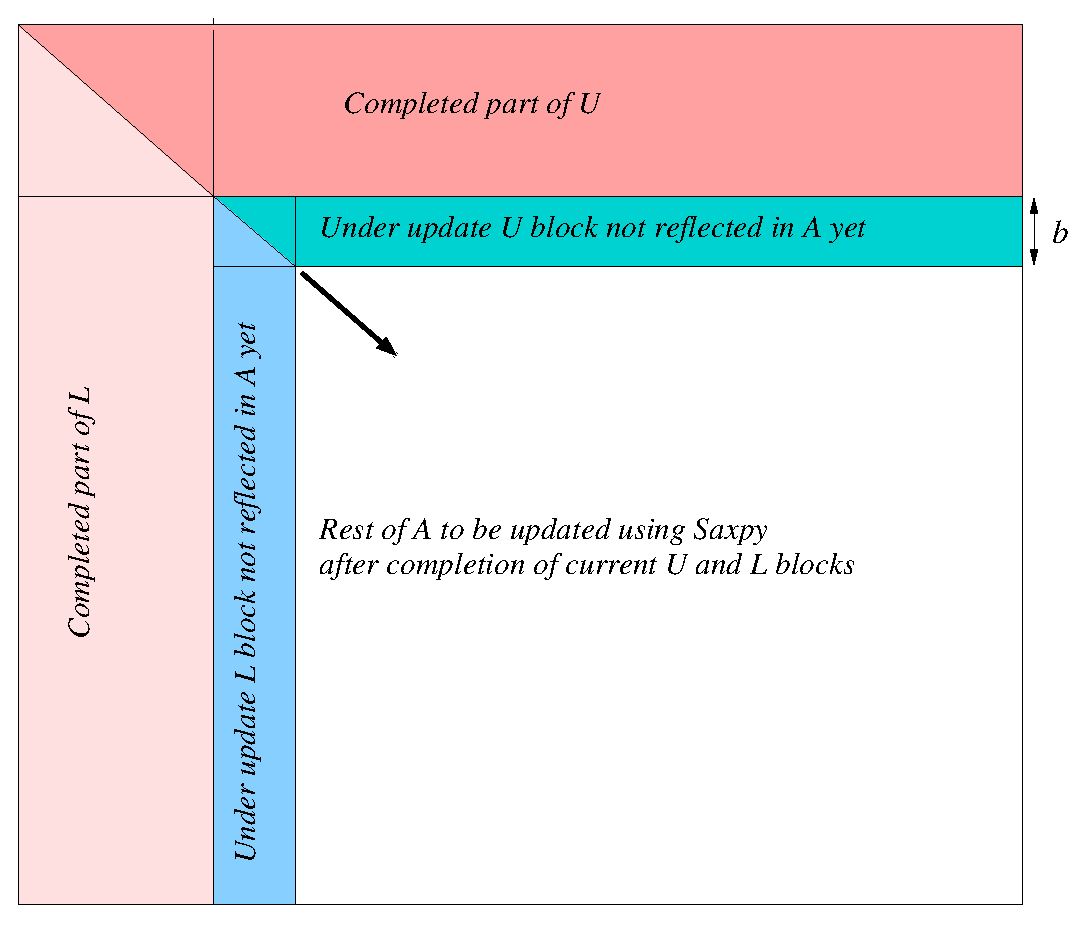
\includegraphics[width=0.9\columnwidth]{Figures/block-LUF-scheme.eps}
	\caption{An illustration of the progression of Block LU decomposition strategy.}
	\label{fig:luf-scheme}
\end{figure}


\begin{algorithm}
	\caption{Block-LU Factorization algorithm}\label{algo:Block-LUF}
	\begin{algorithmic}[1]
		\For{$ r = 0; r < n; r = r + b$}\Comment{Iterate rows in blocks}
		\For{$ r \leq k < r + b$} \Comment{Regular LU iterations}    
		\State $p \gets i\ | \max\limits_{k \leq i \leq n}|\mathcal{A}_{ik}|$
		\State $P[k] \gets p$
		\State $swap(A_k, A_p)$
		\For{$ k + 1 \leq i < n$}
		\State $L_{ik} = \frac{A_{ik}}{A_{kk}}$
		\EndFor
		\For{$ k \leq i < k + b$}\Comment{Update a sliver of rows}     
		\For{$ k + 1 \leq j < n$}
		\State $A_{ij} = A_{ij} - A_{ik} * A_{kj}$
		\EndFor
		\EndFor
		\EndFor
		\For{$ r + b \leq i < n$}\Comment{Saxpy for rest of A}
		\For{$ r + b \leq j < n$}
		\For{$ r + b \leq k < n$}
		\State $A_{ij} = A_{ij} - A_{ik} * A_{kj}$
		\EndFor
		\EndFor
		\EndFor
		\EndFor
		\State $U \gets A$
		\State \Return $P,L,U$
	\end{algorithmic}
\end{algorithm}

Note that the only difference between Algorithm \ref{algo:LUF} and Algorithm \ref{algo:Block-LUF} is of the order of some computation. However, the two algorithms have radically different running times for large $A$ due to divergent cache-usage characteristics when the saxpy part of Algorithm \ref{algo:Block-LUF} from Line $15$ to $18$ is done in small blocks (as in the case of an efficient matrix-matrix multiplication), which Algorithm \ref{algo:LUF} does not permit. This difference is evidence that high performance computing requires careful consideration of the target architecture.

\subsubsection*{Parallel LU Factorization and HighP5 Implementation}
The parallel algorithm for block-LU factorization is the same as that of Algorithm \ref{algo:Block-LUF}. Only rows/columns of the input and output matrices are distributed among processing units for parallel computations. That is, parallel Block-LU factorization is a data-parallel version of sequential Block-LU factorization. Since LU factorization progresses diagonally downward from the top-left corner to the bottom-right corner of the argument matrix; the norm is to partition the matrix using a block-stride partition where each processing unit takes responsibility for interleaving sequence of blocks of rows/columns so that processing units have roughly equal amount of work to do and are active for most of the duration of the computation, maximizing parallelism. Note that it is impossible to evenly distribute the computation burden of LU factorization to all processing units due to the diagonal progression and some steps such as pivot row/column update being restricted to different processing units after data distribution.  

In HighP5, the computation is expressed as a parallel flow of computation stages happening in a hierarchy of logical processing spaces (LPSes) where each space is partitioned into logical processing units (LPUs) doing data parallel computation of the same stages for different data parts, with support for conditional stage executions. A large program unit such as LU factorization with its own LPS hierarchy is called a `Task' in HighP5 which adheres to the SPMD programming model \citep{kamil2013hierarchical}. Listing \ref{highp5-luf} shows the parallel computation flow and partition sections of the HighP5 version of parallel block-LU factorization task. The code for the stages and some other sections of the task are not shown, such as, the data structure definition and binding of input/output with task data\footnote{The full code is available in the end of \cite{yanhaona2024highp5}.}. 

\input{Programs/Block-LUF.p}

The idea of `hardware cognizent' parallel programming in HighP5 is that programmers write a declarative program having tasks each depicting a flow of computation stages happening over a task-specific logical hierarchy of LPSes over different data parts in parallel fashion in LPUs of those LPSes. To generate the executable for a specific target platform, programmers map the LPS hierarchy of individual tasks to the various layers of the hardware architecture called physical processing spaces (PPSes). For example, a PPS can be a CPU core, a NUMA node, a single server rack, a GPU, or even an entire region of a computing network. The physical processing units (PPUs) of a PPS are the uniform parts of a PPS with similar capacities and communication/interaction delays among them. For example, the CPU cores of a single NUMA node are the PPUs of the core PPS, the individual NUMA nodes of a CPU are the PPUs of the NUMA-node PPS, and the collection of nodes in a single server rack of a supercomputer are the PPUs of the node PPS. That is, the entire hardware is described as a rooted hierarchy of physical processing spaces and units. The modeling of a hardware as such is done using a type architecture \citep{Snyder:1986:TAS:17814.17826} called `PCubeS' described in \citep{yanAndrewPCubeS}. Figure \ref{fig:frontier} shows two PCubeS descriptions/models of the Frontier supercomputer \citep{Rajaraman2023}. The first model portrays the hardware as a distributed memory computer that exposes all CPU capacities. The second model is for hybrid CPU+GPU computing that is the focus of another HighP5 compiler. 

\begin{figure*}[htb]
	\centering
	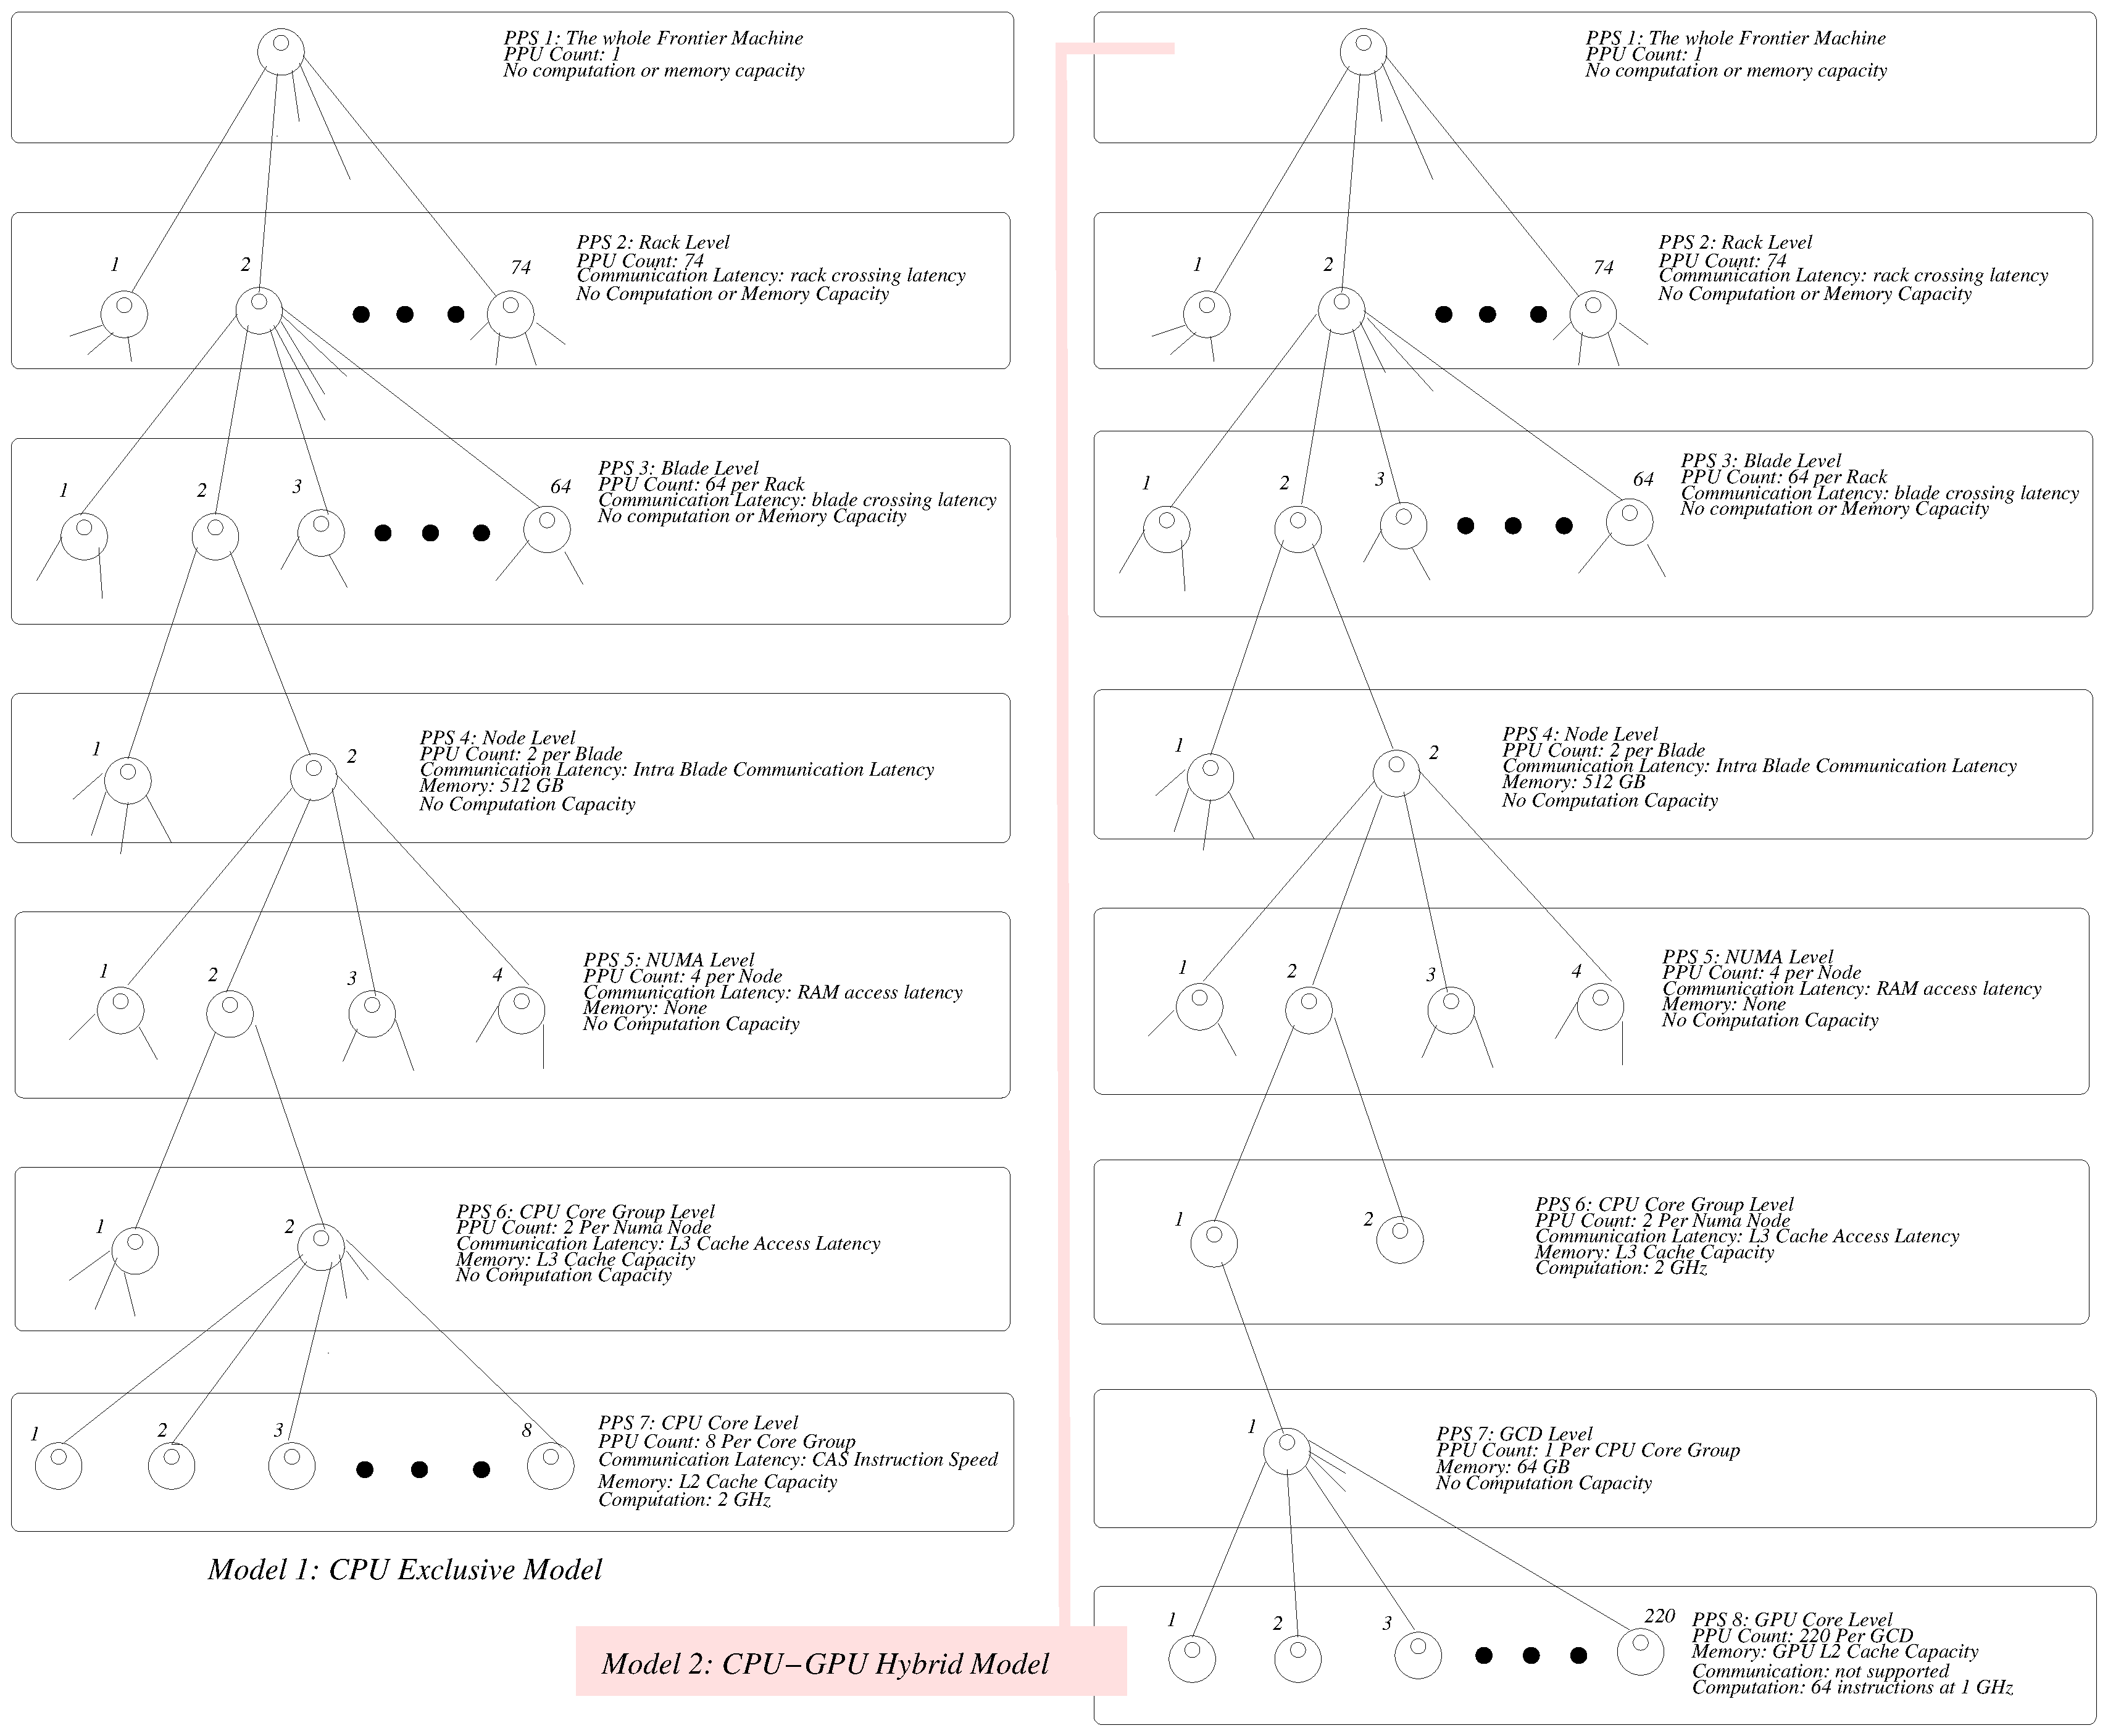
\includegraphics[width=\linewidth]{Figures/Frontier-PCubeS-Models.eps}
	\caption{An illustration of two PCubeS machine models of the Frontier Supercomputer. The depictions expand only one parallel processing unit at each level. Furthermore, details of the communication capacities (exact latencies and transaction bandwidth) have not been shown. }
	\label{fig:frontier}
\end{figure*}

In the Block-LU factorization task of Listing \ref{highp5-luf}, the LPSes are $Space\ A,\ B$ and $C$ as we go downward along the LPS hierarchy. The actual degree of parallelism when executing a HighP5 task depends on the nature of data partitioning defined by programmers in the Partition section of the task, how they map LPSes to PPSes of the target execution platform, and the number of PPUs in the mapped PPSes. The LPUs are multiplexed to the PPUs. Hence, the degree of parallelism increases proportional to the parallel processing capacity of the platform and vary dynamically during a task execution as LPSes of a single task may be mapped to different PPSes. Consider two different mappings of Block LU factorization task's LPSes to the PPSes of Frontier architecture's CPU exclusive model as illustrated below.

\input{Programs/block-luf-mapping-1.map}
\input{Programs/block-luf-mapping-2.map}

In the first mapping, the un-partitioned root LPS, $Space\ A$ is mapped to a single node. Thus, the entire LU decomposition will be confined to a single node where one CPU from each of the $4$ NUMA blocks inside the node will execute the computation stages of $Space\ B$, such as, $selectPivot$, $updateL$, $updateURowsBlock$ of Line $9$, $16$, and $18$ of Listing \ref{highp5-luf}. Finally, $16$ cores per NUMA block will participate in the $saxpy$ computation (Line $33$) for data assigned to the NUMA block.

On the other hand, in the second mapping, $Space\ A$ is mapped to the Rack Level, $Space\ B$ to NUMA Level, and $Space\ C$ to CPU Core Group Level. Therefore, the whole computation will span $64$ blades $\times$ $2$ nodes = $128$ nodes with one CPU per node executing $Space\ B$ computation stages and $8$ CPU cores (one for each core group located within a node) collaborating in $saxpy$ computation assigned to $Space\ C$. This is how programmers generate executables of different nature by changing the mapping configuration for the same HighP5 source code. Programmers specify the intent and compiler handles the implementation, as stated earlier. 

The separation of mapping enables portability across architectures also, where different platform-specific HighP5 compilers generate mapping-appropriate executable. However, for our present discussion, we focus on generating different executables for the distributed memory architecture exclusively. We close this section with a discussion on the nature of a HighP5 executable for distributed memory architectures to understand the general principle of executable generation and consequent challenges the compiler faces regarding properly implementing programmers' decisions.  

\subsection{The Nature of a HighP5 Executable}
\label{subsec:behave-exe}
A major concern with high-level parallel programming languages is the performance ambiguity of program constructs in the generated executable for different target execution platforms. This problem is elegantly explained in Snyder's seminal paper ~\citep{Snyder:1986:TAS:17814.17826} where he shows how the lack of clarity in this regard leads programmer to design sub-optimal parallel programs.

HighP5 tries to overcome this problem by exposing the salient features of the hardware through its hierarchical PCubeS machine model and allowing programmers to control and tune all aspects of parallel program design based on the knowledge of the hardware model. However, to keep programmers' job manageable, the programming model is made \textit{declarative}. Programmers specify which computation stages should execute where in hardware without worrying how the loops and statements are translated. They define what data parts to be available where through the partition specification without knowing the complexities of memory management. Finally, they designate the points where shared/overlapped data parts should be synchronized by setting the LPS transition boundaries in a task's Computation Section without dealing with the nitty-gritty of message passing and synchronization primitives. Given the abstract machine model of the execution platform has detailed capability specification, the cost of all these decisions is clear to the programmers after the mapping of LPS hierarchies of various tasks to the PPS hierarchy of the execution platform during program compilation.

To keep the performance cost assessment true to programmers expectation, the behavior of the compiler generated executable should not deviate from that of a low-level implementation where programmers write the boilerplate codes for all their design decisions. Consequently, the overhead code that compiler adds and the memory footprint of management data structures must be negligible, the implementation of automatic data synchronizations must be optimal, and the compiler should not add any hidden communication/synchronization that the most efficient low-level code could avoid. 

The HighP5 compiler tackles these challenges by generating an optimized C code from HighP5 program that is parallelized using MPI and POSIX threads (Pthreads). This C code is then compiled into the final executable using some nested MPI-C compiler optimum for the target platform. Consequently, the executable for a HighP5 program is an MPI application where each MPI process itself is parallelized using multi-threading. The MPI+Pthread hybrid is chosen as the target to optimize data synchronization. Any data synchronization in the source HighP5 program that is confined within a shared memory segment of the execution platform is implemented using Pthreads synchronization primitives such as semaphores and barriers. Consequently, no communication is involved. When a data synchronization spans across shared memory sub-regions of the distributed memory machine, an appropriate message passing primitive is used from the MPI library.

Therefore, the execution hierarchy has only two levels: MPI processes at upper level hosting POSIX threads under them. The compiler decides about the number of processes and threads based on the LPS-PPS mappings of the various tasks of a HighP5 program. Consider the mapping of Listing \ref{mapping-luf-2} of the block-LU factorization program to Frontier machine. Since shared memory segments are the nodes of the machine, the number of MPI processes for the HighP5 program will be $128$, the total number of nodes within a rack. The number of Pthreads within each MPI process will be $8$, the number of CPU core groups within a node. Here each Pthread will be pinned to the first core of a core group. 

The idea is that each MPI process and Pthread works as a composite PPU controller and executes code and engages in synchronization and communication depending on its role assignments. For example, in block-LU factorization, the topmost LPS, $Space\ A$, is non-partitioned. Consequently, only the first Pthread of the first MPI process will execute the computation stages assigned to $Space\ A$. All Pthreads in all MPI processes will execute computation stages for Space C for LPUs multiplexed to them. Meanwhile, only the thread at core $i$ with $i$ = $0$ (mod $8$) of an MPI process will execute computation stages assigned to $Space\ B$ LPUs. The LPUs are evenly multiplexed to the PPU controllers that have roles in the underlying LPS. 

When there are multiple tasks in the source program, the union of all task's processing requirements and the capacity available in the hardware determine the number of processes and threads. If capacity is restricted, a single MPI process may participate in two different tasks in a lockstep fashion. On the other hand, when more capacity is available, tasks execute concurrently in different MPI processes if there is no inter-task data dependency. In all cases, a single part of the machine is never assigned to multiple tasks simultaneously. The above strategy ensures that runtime parallelism scales proportionally to the parallel processing capacity of the hardware while, at the same time, the overhead of process and thread management is minimal.

In case of multi-task programs, HighP5 offers the notion of tasks executing in an environment consisting of data parts distributed among MPI processes where execution of a task modifies parts of the environment. The MPI processes last for the entire runtime of the program, the Pthreads inside the processes are cleaned up and spawned again based on the nature of individual tasks' LPS hierarchy. When there are data dependencies among tasks, a subsequent task gets the up-to-date data left in the environment by earlier tasks. Therefore, there is no accumulation and re-distribution of data during transitions between tasks unless the dependent task's data distribution specification is different from how the data is currently residing in the collective MPI environment. Figure \ref{fig:runtime} illustrates the runtime model of an HighP5 executable. Here, the garbage collector kicks in at the end of the execution of each task to cleanup management data structures and intermediate outputs of the task not needed any further.  

\begin{figure}[htb]
	\centering
	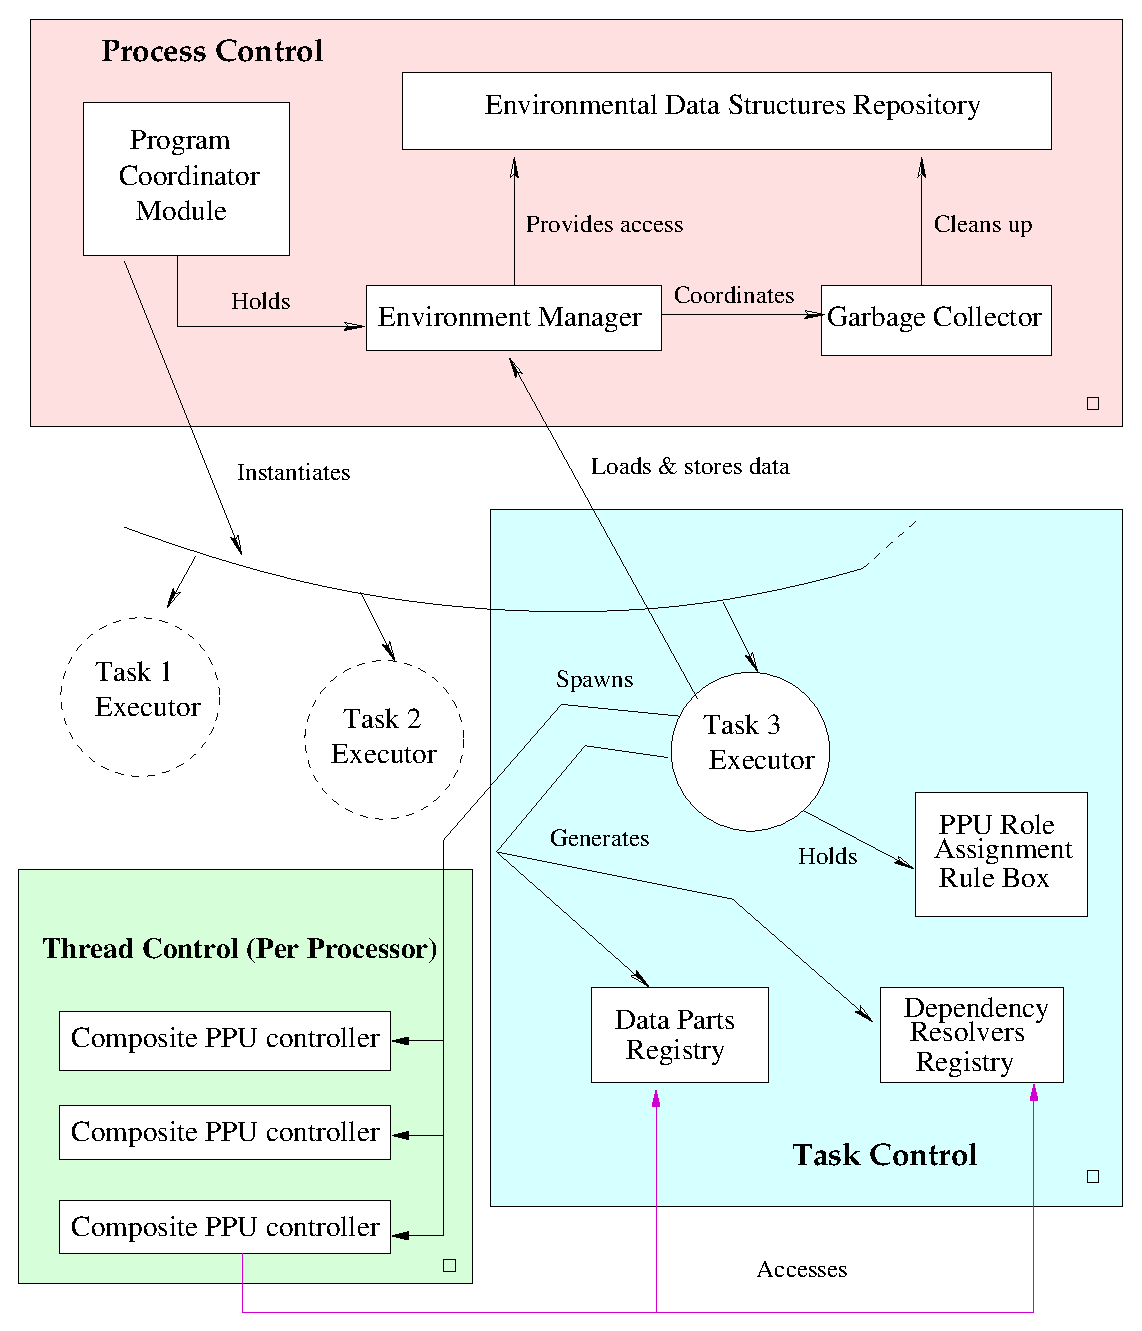
\includegraphics[width=\columnwidth]{Figures/compilation/runtime-model.eps}
	\caption{The runtime process model of HighP5 executables. }
	\label{fig:runtime}
\end{figure}

Individual composite PPU controller threads for a task are basically flow executors that traverse a flow template and execute a computation stage or skip it   depending on its LPS role assignments. For each computation stage, the data parts for the underlying LPU come from the shared data parts registry that is managed by the task executor. As a flow executor reaches a point that requires a synchronization/communication, it retrieves relevant primitives from the data dependency resolver registry and invokes the appropriate sync function. The execution model of such a thread is illustrated in Figure \ref{fig:ppu-controller}.   

\begin{figure}[htb]
	\centering
	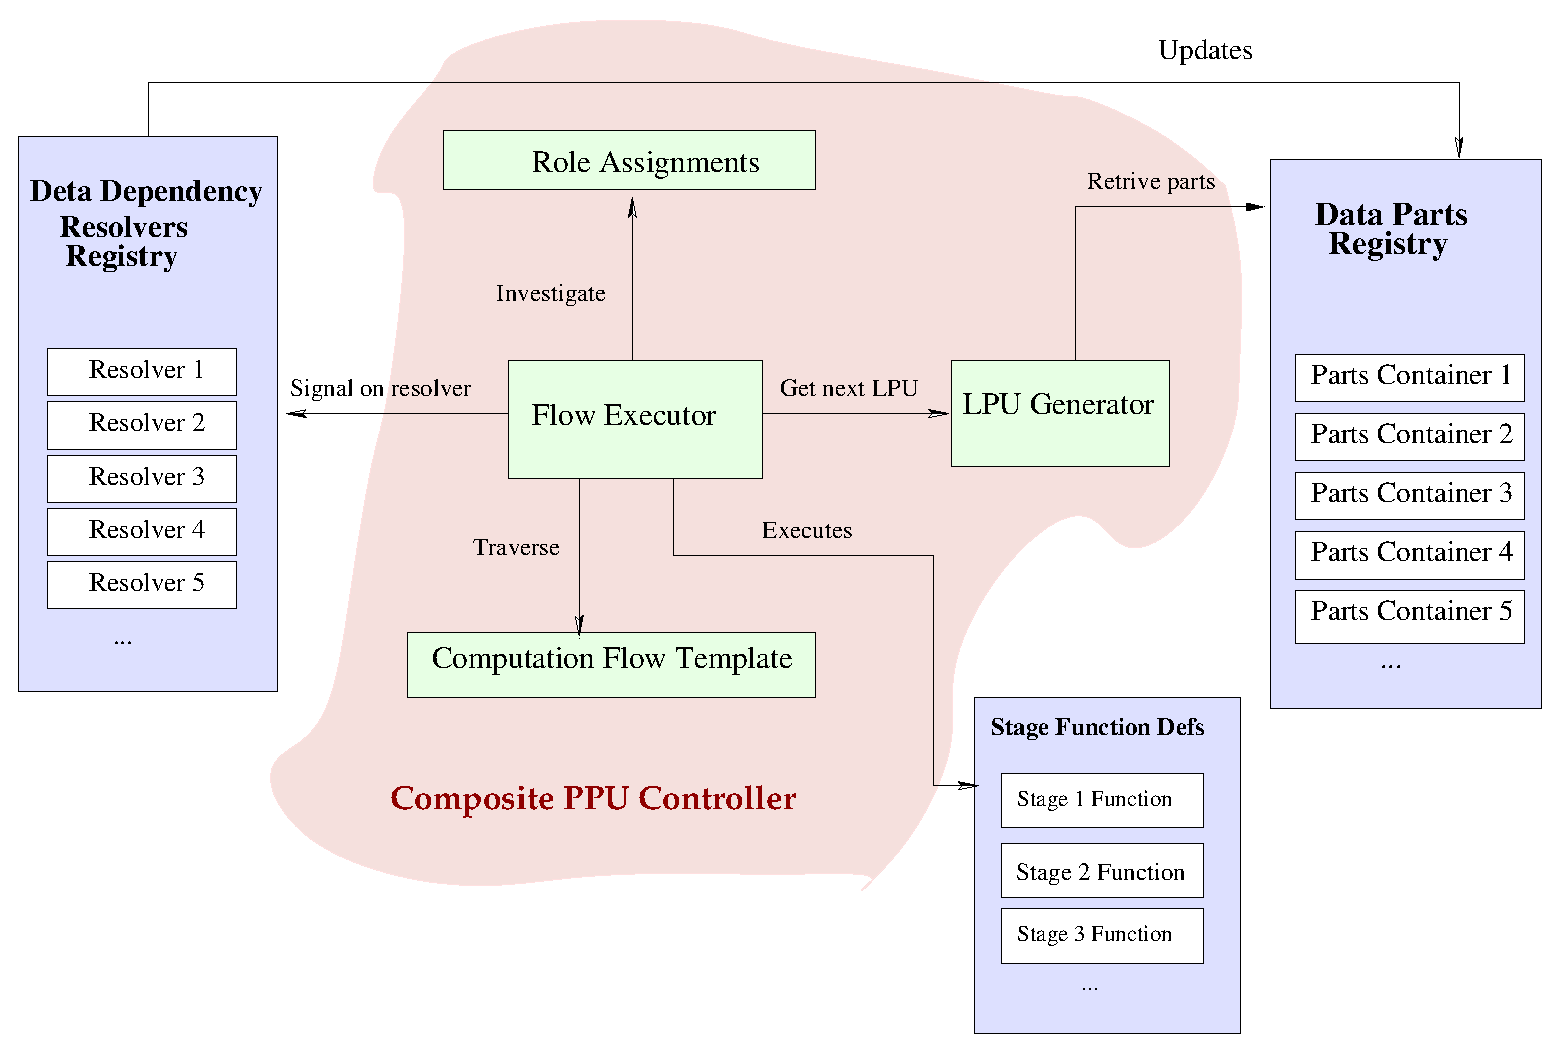
\includegraphics[width=\columnwidth]{Figures/compilation/ppu-controller-model.eps}
	\caption{The architecture of a composite PPU controller thread.}
	\label{fig:ppu-controller}
\end{figure}

Finally, note that the programming paradigm encourages programmers to choose data distribution and computation assignment based on their understanding of the PCubeS description of the target platform that exposes all layers of the interconnection network in the machine and cache-organization inside individual nodes. Consequently, implementing data movements from RAM to caches as programmer-intended and confining communications within only relevant nodes are part of compiler's responsibilities. All these along with a careful translation of computation stages and synchronization/communication directives from the HighP5 program to the hybrid MPI+Pthread intermediate is essential to exhibit a performance similar to a hand-written optimized low-level code. 
	
\section{Overview of the Compiler}
\label{sec:compiler-overview}
HighP5 offers a paradigm of parallel programming in which the same source code is portable to different architectural platforms. Programmers write the source code using abstract LPS hierarchies to have a flexible declarative program that can be mapped appropriately to platform-specific features to derive an efficient executable for the target platform. To enable this feat, the HighP5 compiler has the breakdown where the compiler front-end doing lexical, syntax, semantic, and static analyses generates an intermediate form using the source code exclusively, ignoring the programmer-supplied mapping configuration. The back-end compiler has the understanding of architecture-dependent interpretation of PPS hierarchy of the platform. The mapping configuration is fed to this back-end for further analyses before code generation can begin. For the distributed-memory HighP5 compiler this responsibility breakdown is illustrated in Figure \ref{fig:compilation-breakdwon}.    

%\begin{figure}[htb]
%\centering
%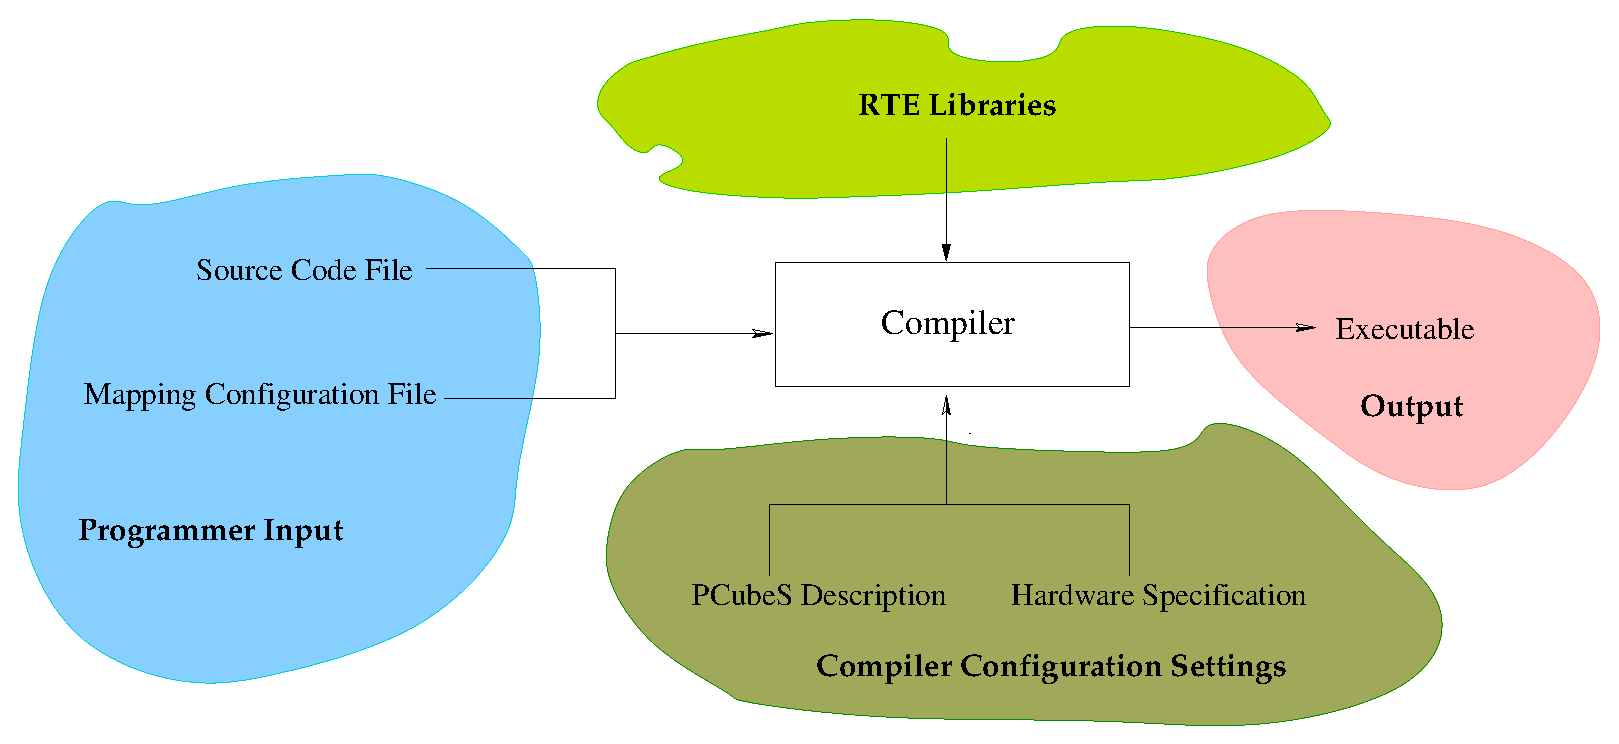
\includegraphics[width=\columnwidth]{Figures/compilation/compilation-broad-picture.eps}
%\caption{A schematic diagram of the compilation process in terms of input/output.}
%\label{fig:compilation-broad-view}
%\end{figure}

\begin{figure}[htb]
	\centering
	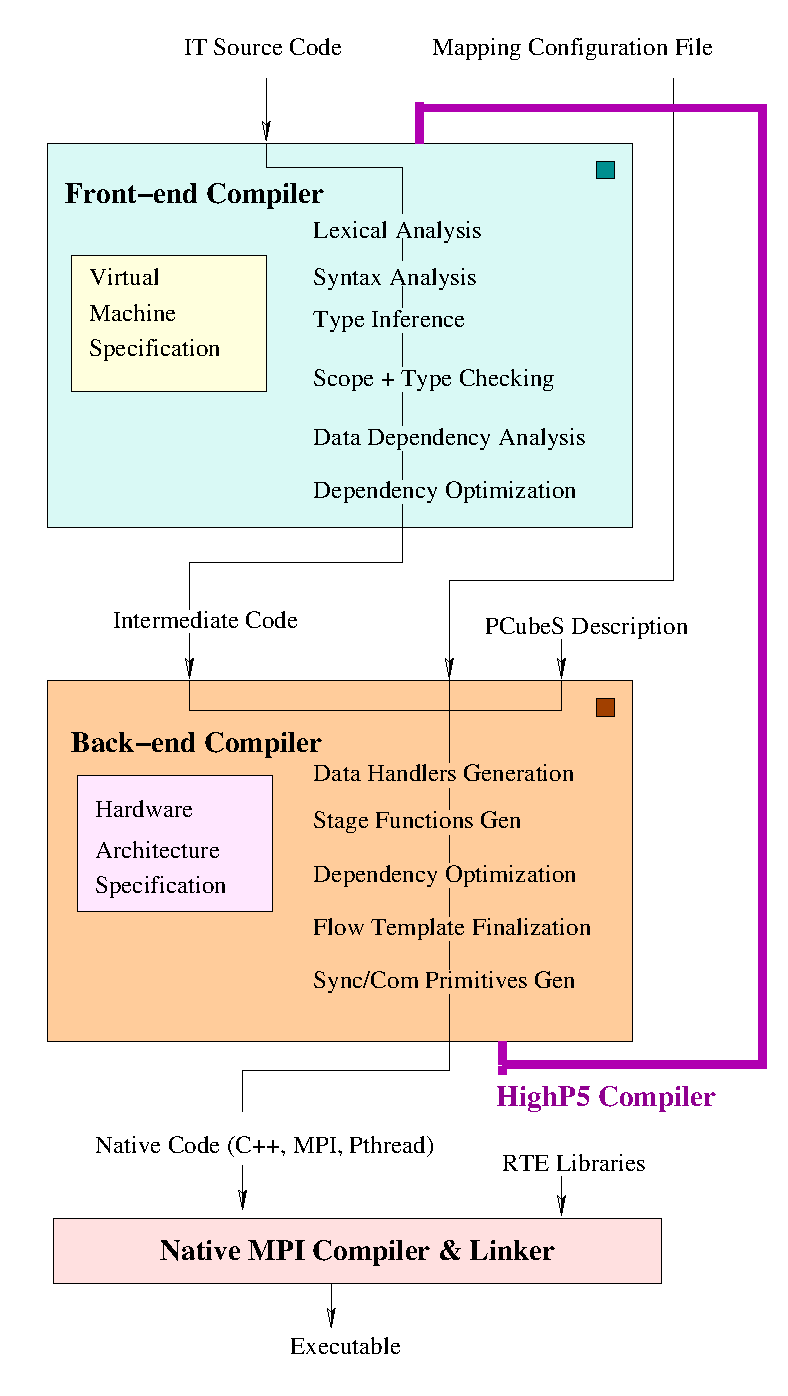
\includegraphics[width=0.9\columnwidth]{Figures/compilation/compiler-breackdown.eps}
	\caption{Front-end/Back-end breakdown of the compiler.}
	\label{fig:compilation-breakdwon}
\end{figure}

HighP5 is a partially and strongly typed language. Only the types of `task global' variables that are shared across processes and stay alive for the duration of a task execution are defined in a specific `Define' section of a task and the types of all remaining local and global variables (including I/O) are inferred. Consequently, there is a type inference step after syntax analysis that kicks of the semantic analysis phase. The concept of partial typing is illustrated in Listing \ref{highp5-luf-stages} showing the Define and key parts of the Stages section of block-LU factorization task. The type inference is done using a fixed-point calculation. That traverses the abstract syntax tree of the whole program and infers types of new variables and expressions from that of those whose types are already known. The traversal is repeated as long as new types are discovered or it ends with no further type discovery.   

\input{Programs/block-luf-stages.p}

If type inference is successful, then scope + type checking starts, which is no different from how this step is done in other languages. However, afterward, the compiler needs to invoke sophisticated static analysis to determine the optimum read-write dependencies among compute stages for shared data. Note that the front-end compiler cannot determine how to resolve those dependencies as it operates using the notion of logical LPS hierarchies of tasks. However, it can eliminate many redundant dependencies based on tasks' partition specifications and placement of stage functions in LPSes. The final output of the front-end compiler is a collection of abstract flow templates for individual tasks, the abstract syntax tree for the coordinator program that launches tasks, intra and inter-task data dependency graphs, and symbol tables for various scopes.     

The back-end compiler understands how to deal with shared memory parts of individual nodes of the distributed memory machines, the logic of pinning threads to processing cores for better cache utilization, and the logic of pair-to-pair and group communication in a generic way. Configured with the PCubeS description of the specific target execution platform and supplied with programmers' mapping configuration file, it is able to translate the generic rules to specific C code parallelized with MPI and Pthreads. The execution mechanism of composite PPU controller threads as shown in Figure \ref{fig:ppu-controller} is uniform for all tasks for a specific type of execution platform architecture and, henceforth, comes from a native format runtime environment (RTE) library. The back-end compiler applies complex multi-step analyses to populate the data parts and data dependency resolver registries, configure roles for PPU controller threads and MPI processes, and generate C functions for computation stages and the flow templates. 

Similarly, the environment management mechanism and garbage collection logic of Figure \ref{fig:runtime} are parts of the common runtime. The back-end compiler generates the program coordination function (works as the main function of the final MPI program), task executor functions for individual tasks (handle initialization of threads and registries), and environment instructions that link inter-dependent tasks and I/O operations. The advantage of adopting environment instructions for linking is that individual task compilations can be treated as independent of one another that made code optimization easier. 

The key concerns related to efficiency of the generated executable is as follows:
\begin{enumerate}
	\item \textbf{Task Data Management}: involves efficient data handlers generation for Data Parts Registry and data access optimization.
	\item \textbf{Flow Execution Code Generation}: involves appropriate code generation for stage functions and cache-aware multiplexing and iteration of LPUs.
	\item \textbf{Synchronization and Communication}: involves data dependency optimization, proper sync/communication primitive generation, and maximizing computation-computation overlaps.
	\item \textbf{Environment Management}: involves generating proper environment instructions and handler code.
\end{enumerate}
Among the above, the first three are dealt with on individual tasks basis and the last by considering inter-task dependencies. We cover these topics in detail in the following sections.

\section{Task Data Management}
\label{sec:task-data-mgmt}
Key aspects of managing the data relevant to a task is to interpret and translate the hierarchical data distribution specifications found in task's Partition section, generating code for allocating data parts and LPU metadata inside MPI processes and populating the parts, and accessing the parts during stage executions over LPUs by composite PPU controller threads. We discuss these concerns in the following subsections.

\subsection{Handling Hierarchical Data Distributions}
\label{subsec:data-distro}
HighP5 supports four standard data distribution specifications for partitioning an array dimension: block-size, block-count, stride, and block-stride. Let us investigate their behavior on an array dimension of length $N$.
\begin{enumerate}
	\item $block$-$size(n)$ divides $N$ into $\frac{N + (n - 1))}{n}$ blocks each owning $n$ consecutive indices along the dimension, except for the last block which can be smaller.
	\item $block$-$count(c)$ divides $N$ into $c$ consecutive index blocks each of size $\frac{N + (c - 1)}{c}$. Again, the last block can be smaller if $c$ does not divide $N$.
	\item $stride(n)$ divides $N$ into $n$ partitions where the $i^{th}$ partition owns the indices $i, n + i, 2n + i, 3n + i, \cdots$.
	\item $block$-$stride(b, n)$ divides $N$ into $n$ partitions where the $i^{th}$ partition owns the indices $(bi, bi + b - 1), (bni, bni + b - 1), (2bni, 2bni + b - 1), \cdots$. Here $(a,b)$ means the inclusive range from $a$ to $b$.
\end{enumerate}
For a multidimensional array, different dimensions can be partitioned using different data distribution schemes in each LPS. These four data distributions are well known from the days of FORTRAN D ~\citep{10.1007/BFb0038655} and cover most parallel programming problems. For irregular data structures, such as a graph, the recommendation is to use their array representations (e.g., adjacency matrix, CSR, COO) and partition the array(s). Finally, programmers can left some array dimensions un-partitioned in specific LPS or replicate content along some dimensions. 

Note that block-size and stride distributions are special cases of the block-stride distribution function. In all four cases, we can describe the indices of a dimension assigned to a specific LPU by the partitioning scheme as an interval function of the form $f(\beta, \eta, \rho, \zeta)$. Here $\beta$ is the starting index, $\eta$ is the ending index, $\rho$ is the periodic interval, and $\zeta$ is the index range within a periodic interval that belongs to the LPU under concern. Given partitioning is hierarchical, the interval function of the LPU divides the index range assigned to its ancestor LPUs in upper LPSes. If we order the LPSes that partition an array dimension from lower to upper positions in the hierarchy as $l_1, l_2, l_3, \cdots, l_L$ and use the notation $f_{l_i}$ to designate the data distribution function at $l_i$ then the hierarchical interval range function $\delta_{l_1}$ for the lowest LPU can be expressed as a function composition as follows: 

\begin{equation}
	\label{eq:single-dim-part}
	\delta_{l_1} = f_{l_1} \circ f_{l_2} \circ f_{l_3} \cdots \circ f_{l_L}
\end{equation}

Figure \ref{fig:partition-function} illustrates the composition of data distribution using a two layer hierarchy where the upper LPS uses block-stride partitioning and the lower LPS uses block-count partitioning functions.

\begin{figure*}[htb]
	\centering
	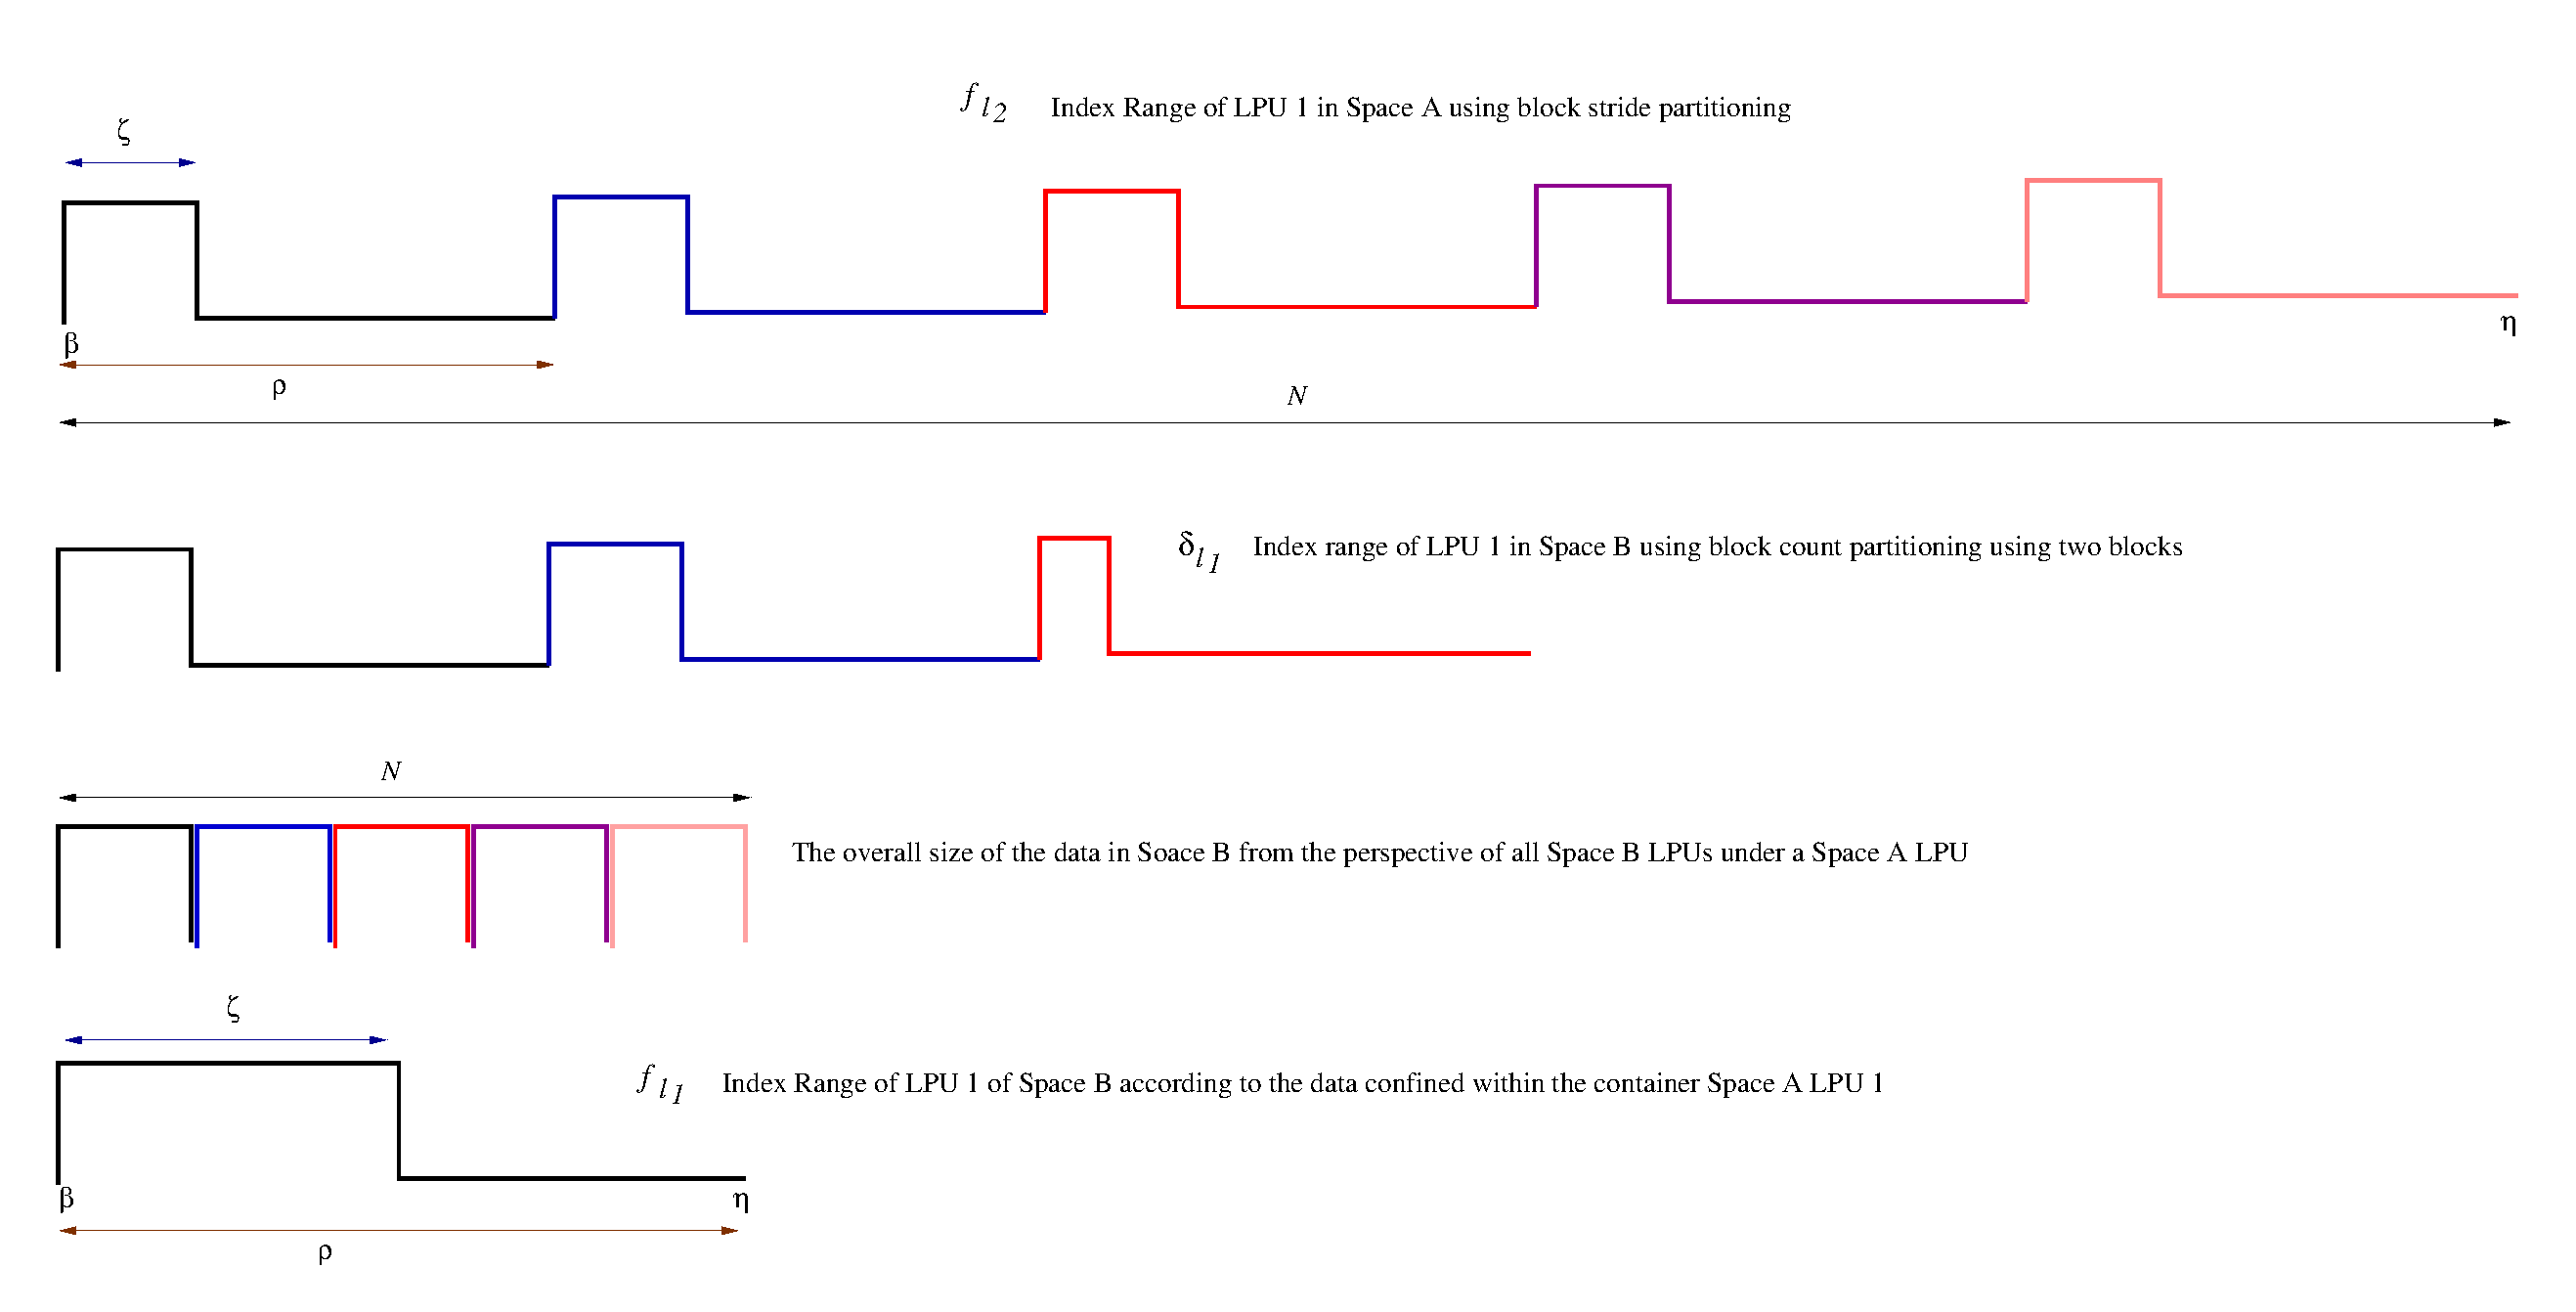
\includegraphics[width=\linewidth]{Figures/interval-function.eps}
	\caption{An illustration of nested data partition using a two layer hierarchy where Space A is the upper and Space B is the lower LPS.}
	\label{fig:partition-function}
\end{figure*}

For a $D$ dimensional array, the index ranges allocated to the LPU for all dimensions can be expressed as the sum of Equation \ref{eq:single-dim-part} as follows:

\begin{equation}
	\label{eq:array-dims-part}
	\Delta_{l_1} = \sum_{d = 1}^{D}f_{l_1}^d \circ f_{l_2}^d \circ f_{l_3}^d \cdots \circ f_{l_L}^d
\end{equation}

Here, the superscript for the distribution functions indicates that the functions can be different for different dimensions. Note that values for the configuration parameters for the component functions of a hierarchical distribution configuration are available mostly at runtime. Therefore, the compiler generates hierarchical data structures that are initialized using command-line parameters, execution-time configuration (e.g., MPI process count), and metadata from input files (e.g., dimension lengths of individual arrays) during the launch of a task executor (Figure \ref{fig:runtime}).  .

\subsection{Memory Allocation in MPI Processes}
\label{sub-sec:array-aloc}
HighP5 is an array-based language in the sense that the prime focus of data distribution is arrays. Buffer allocation for lists and other structures is simple as they are replicated across LPUs of an LPS. Consequently, a single whole copy can be used for all LPUs' computation stages inside an MPI process. Buffer allocation for array parts and loading (from input files) and retrieving (from remote memory locations) array items in those buffers requires ingenuity.

If $f(\beta_i^j, \eta_i, \rho_i, \zeta_i)$ is the interval function for a particular LPU $l_j$ for partitioning a dimension $i$ of an array $A$, the total number of index points along that dimension, $\iota_i^j$, for $l_j$ follows the equation:
\begin{equation}
	\label{eq:1d-element-count}
	\iota_i^j = \zeta_i \frac{\eta_i - \beta_i + 1}{\rho_i}    
\end{equation}
If $A$ is $D$ dimensional then the buffer capacity requirement for the part of $A$ assigned to $l_j$ is:
\begin{equation}
	\label{eq:lpu-capacity-req}
	I_j = size(A.elementType)\prod_{i = 1}^{D}\iota_i^j    
\end{equation}

As data distribution is hierarchical, the index points calculation for a lower level LPU $l_j$ can be done by repeatedly applying Equation \ref{eq:1d-element-count} from topmost ancestor LPU $l_1$ down to $l_j$ by treating $\iota_k - 1$ as $\eta_{k+1}$ for all $1 \leq k < j$. The overall buffer capacity requirement for a single array's parts for all LPUs of an LPS multiplexed to an MPI process can be computed by summing up Equation \ref{eq:lpu-capacity-req} for all LPUs. The total capacity requirements calculation can be optimized by utilizing the fact that consecutive LPUs are multiplexed in a single PPU controller process. Consequently, LPUs' data distribution interval functions can be combined as follows:

\begin{equation}
	\label{eq:interval-composition}
	\sum_{j = 1}^{j = n} f(\beta_i^j, \eta_i, \rho_i, \zeta_i) = f(\beta_i^1, \eta_i, \rho_i, n\zeta_i)
\end{equation}

The compiler generated intermediate C code utilizes this last equation to determine the buffer capacity requirement for each array inside an MPI process in constant time and allocates the buffer. Allocating all the parts of an array needed inside an MPI process as a single contiguous buffer has the advantage that when garbage collection takes place, the entire buffer can be freed in a single step, eliminating all associated data parts.

Note that programmers may define an LPS hierarchy where two different LPSes from different branches of the hierarchy requiring the same array for their computation stages but using different data distribution strategies. If some LPUs of both these LPSes are multiplexed to a single MPI process then there is no feasible way to maintain a single buffer for all data items the process needs to hold. Furthermore, such an attempt reduces the chance of parallel computation. Therefore, an MPI process maintains a separate buffer for each distinct maximal path from the root of the partition hierarchy to the lowest that requires the underlying array. Buffer synchronization within a process for a pair of LPUs not related via an ancestor-descendant relationship is treated as a communication problem.

An important aspect of a path in the LPS hierarchy is that each LPS along the path is dimensional. Consequently, the LPUs can be hierarchically ordered based on the number of partitions in the LPSes and the position of the LPU in the hierarchical order, which gives us a hierarchial LPU ID for each LPU. An array part that is needed by a particular LPU can be given a hierarchical multi-dimensional part-ID derived from the LPU ID. The compiler utilizes this fact to generate code for a part-ID-tree construction for individual buffers. The leaves of the tree refer/point to unique data parts, each pointing to the beginning of a continuous stretch of indices in the buffer. That is, the elements of a single data part are always located in consecutive indices regardless of how the partition configuration may have re-ordered the indices of the original array. This treatment is important to ensure that the data for an LPU computation can fit in the memory of the PPU programmers used for the mapping and that there is no opaque data access overhead that cannot be easily debugged.    

The portion of the Data Part Registry code (Figure \ref{fig:ppu-controller}) that belongs to the RTE library is extended by compiler-generated code for buffer allocation, part-ID-tree construction, and parts retrieval by IDs for each array and LPS combination. Collectively, they form a data parts container and the registry holds a map of such containers. For the first HighP5 task that needs an array $A$ for its computation, data items are read into the allocated buffer from input files concurrently in all MPI processes collectively by PPU controller threads as part of the registry initialization process. Initialization of the registry for any subsequent HighP5 tasks that require $A$, data item loading involves cross-task communications, which we discuss later. 

\subsubsection{LPU Metadata Management}
\label{subsec:lpu-data-mgmt}
since HighP5's hierarchical machine model exposes all physical processing spaces (PPS) and their units (PPU), programmers are encouraged to choose partition parameters that promote best cache utilization, optimize data transfer cost, and maximize parallel execution. Consequently, the number of LPUs can be quite large in the lower LPSes. To give an example, if the block-size $b = 64$ and the argument matrix is $10240 \times 10240$ in the block-LU factorization problem of Listing \ref{highp5-luf}, then the number of LPUs in Space B will be $(\frac{10240}{64})^2 = 256000$ and the number of LPUs for each sub-partition of Space B LPU will be $\frac{10240}{64}=160$. Therefore, a straightforward implementation of MPI processes maintaining a list of LPUs for each LPS they are responsible for and executing computing stages in Pthreads by traversing the list may have a disastrous effect. The LPU tracking lists themselves can overwhelm the memory capacities of the computing nodes. The clever work around this problem is to port translated partition specifications of a task of the source program directly into the intermediate C code.

The compiler generates statefull classes for generating LPU metadata for various LPSes whose instances are created with runtime partition configuration and metadata related to relevant data structures for each composite PPU controller thread. A composite PPU controller thread has multiple static IDs (or ranks) for various PPSes based on the exact hardware units of the execution platform's PCubeS model they represent. As a thread enters/re-enters a new LPS in the flow execution template of the task, it initializes/resets an LPU iterator in the LPU generator with its associated PPU IDs. Here, the PPU IDs are used by the generator class to determine which LPUs are being multiplexed locally and assigned to the threads. The LPU generator computes and returns the next LPU each time the thread asks for one until the LPUs of the thread are exhausted. 

An LPU generation involves calculating an LPU ID, deriving various data part IDs from the LPU ID, setting up data part pointers to allocated buffers, and generating part metadata (e.g., a data part size and dimension ranges). It may appear that computing and recomputing LPUs in this manner is costly. However, compared to the execution cost of functions for computation stages, the LPU generation cost is typically insignificant. Furthermore, all calculations related to LPU generation are integer computations that are further inlined in a single function by the final MPI-C compiler. Thus, this strategy effectively eliminates memory footprint for LPU metadata management in exchange for some integer computation overhead.  

\subsection{Data Access During LPU Computation}
\label{subsec:lpu-data-access}
The logic for accessing data parts while executing a computation stage on a particular LPU is rather simple. Since LPU metadata has data part IDs for each array part, it is possible to search the associated part-id-tree in the Data Parts Registry to retrieve the location pointer to the buffer for that data part using the hierarchical part ID. This is done during the generation of the LPU. Subsequent read-write on the array as part of the execution of the computation stages is done using that location pointer. Figure \ref{fig:part-retrieval} shows how the part retrieval process works for Space C LPUs of the block-LU factorization code of Listing \ref{highp5-luf} during the execution of `saxpy' computation stage.

\begin{figure*}[htb]
	\centering
	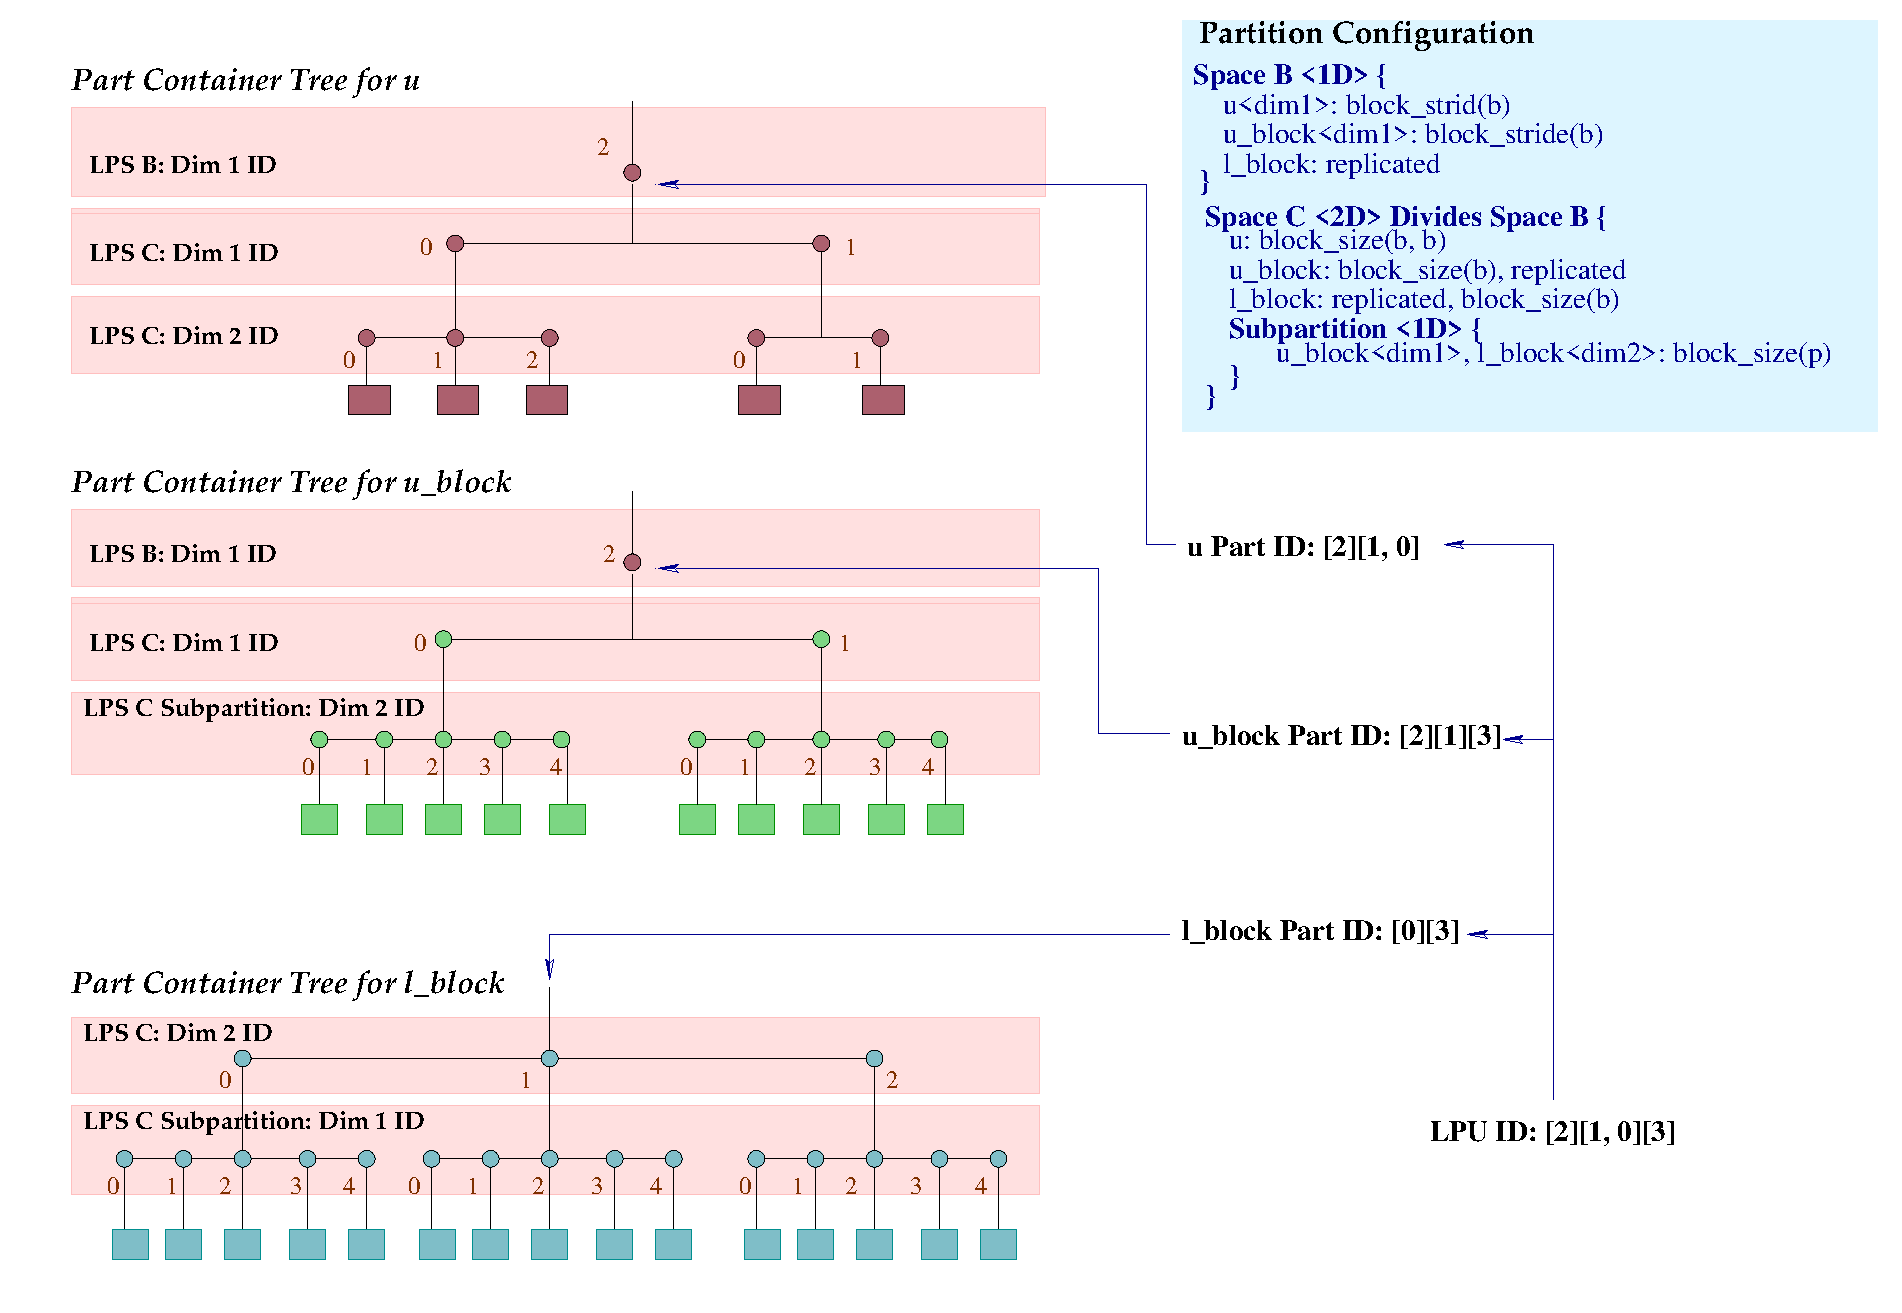
\includegraphics[width=0.70\linewidth]{Figures/compilation/part-container-tree-search.eps}
	\caption{An illustration of the process of retrieving data parts from Data Parts Registry using an LPU ID during block-LU factorization.}
	\label{fig:part-retrieval}
\end{figure*}

For task-global scalars and list type variables, a single global data structure instance is generated by the compiler that holds their memory references. All composite PPU controller threads access these variables through that single instance.

\section{Flow Execution Code Generation}
\label{sec:flow-exec-code-gen}
From a high-level perspective, the flow execution code generation is the activity of merging the compute stages of the Stage section of a task (e.g., Listing \ref{highp5-luf-stages}) to its Computation section (e.g., Listing \ref{highp5-luf}) to have a pthreads `run' function that every composite PPU controller thread executes. That different threads will operate on different data is ensured by LPU multiplexing based on PPU IDs. Since HighP5 stage functions are type polymorphic, the compiler often generates multiple type-specific C++ implementations for a single stage function based on its calling context. The parameters for the C++ functions are modified to only access the current LPU data structure, task specific metadata, and PPU controller specific information. This modification is essential to simply synchronization and communication code generation which we discuss later. Listing \ref{luf-thread-run-part} shows a part of the generated thread run function of the block-LU factorization task that invokes the `selectPivot' stage as an illustration of the stage execution logic.

\input{Programs/c-code/block_luf_part1.cc}

There are several subtle performance issues that make code generation for a task's flow executor a more involved process than just invoking translated C++ stage functions on multiplexed LPUs.

First, given programmers are encouraged to fully utilize the various cache layers exposed by the PCubeS description of a target platform, the LPU hierarchy can be quite deep in a task, with small data parts inside the lower level LPUs. Consequently, the ratio between the amount of calculations as part of a stage computation and that for generating the LPU metadata can be quite low, giving us a large computation overhead. The compiler applies several optimizations to mitigate this problem. First, LPU metadata generator uses the same LPU object and only updates its revelant ID parts in the LPU iteration process described earlier as the PPU controller proceeds from one LPU to the next. Second, iterators are maintained over each associated part-ID-tree also to avoid traversing the trees from the root every time only a small part of the LPU ID changes. In fact, quite often some data part references remain the same as computation flows from LPUs to LPUs. Finally, LPUs are multiplexed to PPU controllers as continuous swaths to minimize up-down movements along part-id-trees as the iterators advance due to LPU ID changes.

Then, programmers may have redundant LPS transitions in the Computation section of the task that translated as specified will increase overhead. Hence, the compiler tries to reorder stage invocations to fit multiple stage function invocations inside an LPU iteration loop as long as there are no data dependencies precluding such reordering.

Finally, since the computation stages (see Listing \ref{highp5-luf-stages}) are written in a manner oblivious to the data distribution specification which may reorder array indices arbitrary many times (e.g. in Space B of Listing \ref{highp5-luf}), careful consideration is needed to minimize the overhead of transforming an array index to its storage location in the generated C++ stage functions. 
That HighP5 computation stages use declarative multi-index loops comes in handy in this regard. Consider the `saxpy' computation stage in Listing \ref{highp5-luf-stages} (from Line 46 to 54). The compiler knows that the row indices are reordered for $u$ and $u\_block$ but column indices remain unaltered. Therefore, it generates a doubly-nested for loop with row traversal in the outer and column in the inner loop to reduce recalculation of data to storage index mapping. This is illustrated in the truncated version of the generated code shown in Listing \ref{luf-saxpy-C}.
\input{Programs/c-code/block_luf_part2.cc}
Here, the conversion from data to storage index for $u$ and $u\_block$ happens from Line 12 to 18. This strategy of loop ordering based on the data distribution saves computations most of the time. However, when an array index is not a part of a declarative loop, then the index transformation must be done in place, as needed for the index `pivot' in Line 23 of Listing \ref{highp5-luf-stages}.   

\section{Synchronization \& Communication}
\label{sec:sync-primitives}
In HighP5 programming model, synchronization and communication for shared data within a task only happen at LPS transition boundaries. Consequently, the compiler only focuses on resolving read/write dependencies among computation stages at LPS transitions by inserting proper synchrnization/communication code. This is a multi-faceted effort where some of the decisions are made by the compiler front-end, the back-end, and, surprising, even by the RTE initializer. An elaborate approach is implemented in this regard since the optimization of synchronization and, in particular, communication is pivotal for good performance in distributed memory environments. 

Note that all LPS transitions may not be explicit in the source code. Hence, the front-end compiler transforms the computation flow specification of the task into a revised intermediate from where all LPS transitions are explicit. This often results in insertions of dummy computation stages in the flow that are only added to expose all read-write data dependencies that are modeled as directional arrows between computation stages. Subsequently, the front-end compiler applies a technique that we call `lifting', to move dependencies between stages inside repetition loops and conditional blocks (e.g., `selectPivot', `updateURowsBlock' of Listing \ref{highp5-luf}) and stages outside them (e.g., `copyUpdatedUBlock') to LPS transition positions that minimize the invocation of dependency resolution routines without violating accuracy. Finally, it investigates all data dependency arrows and removes any redundencies being found. Without the knowledge of the PCubeS description and the mapping of LPSes of the task to PPSes of the hardware, The front-end compiler cannot determine whether a dependency requires synchronization or communication, and how the participants for a dependency resolution should be selected. Therefore, dependency optimization from the front-end compiler ends here. 

The back-end compiler compares the PCubeS description of the hardware with the programmer-provided mapping file to determine the \textit{confinement} of a data dependency requirement. A confinement is a branch of the PPS hierarchy rooted at the closest ancestor PPS connecting the source and sink of a data dependency arc (Note that the source and sink can be the same PPS when the related LPSes are mapped to the same PPS or a single LPS used overlapping data partition among its LPUs.). Depending on how LPSes are mapped to the PPSes, confinements may be internal to individual MPI processes or spanning multiple processes. If a confinement is internal to an MPI process and both the source and sync LPSes are using the same data buffer then the data dependency is a synchronization requirement. Otherwise, it is a communication requirement. 

\subsection{Resolving Synchronization Dependencies}
\label{subsec:sync-dependencies}
Synchronization dependencies are resolved by inserting code that does Pthreads barrier synchronizations in appropriate places in the flow execution template. Here, the number of sync primitives and the participant count for each of them is deterministically resolved using the hardware's PCubeS description. Initialization of all sync primitives is done by the task launcher (Figure \ref{fig:ppu-controller}) before the PPU controller threads are started. Line 20 to 26 of Listing \ref{luf-sync} illustrate the technique of synchronization for update dependency between the `updateUColsBlock'  and `saxpy' stages of Listing \ref{highp5-luf}. The idea of lifting is apparent here. Although the stages are in two different repeat loops in the source code, the synchronization is placed outside the loops in the interim C++ code. The synchronization from Line 36 to 39 of Listing \ref{luf-sync}, on the other hand, is for the update of $u$ inside the `saxpy' stage impacting `copyUpdatedUBlock'of Listing \ref{highp5-luf}, which could not be lifted beyond the Space B LPU iterations without violating accuracy.
\input{Programs/c-code/block_luf_sync.cc}

The way the synchronization code is generated, a semaphore-based implementation would be possible as an alternative to barrier synchronization that would foster higher independent progress among the relevant PPU controller threads. However, our observation so far in all target platforms is that semaphore and conditional variable based sync primitives scale poorly compared to basic barrier synchronization as the number of participant threads increases. Consequently, both signaling and waiting internally end up waiting on the same barrier primitive. Finally, note the existence of the clause \textit{uStage21No4 > 0} in the signaling part. As the source for the dependency may be different PPU controller threads in different iterations, whether a thread actually executed the relevent computation stage is stored in a variable to control the signaling. This is why every stage function returns a status at exit as shown in the last line of Listing \ref{luf-saxpy-C}.  

\subsection{Resolving Communication Dependencies}
\label{subse:comm-dependencies}
When a data dependency resolution involves communications then -- unlike a synchronization requirement -- we not only need to know the overall participants but also the individual source-destination pairs and the exact data to be exchanged among each pair. These additional burdens make communication handling far more sophisticated than synchronization.

The only easy scenario is the sharing of update of scaler and and fully-replicated data structures. An MPI broadcast among all processes is sufficient. For any array that is partitioned one or more times in the LPS hierarchy, following related questions need to be answered:
\begin{enumerate}
	\item How does an MPI process determine the other MPI processes it has to communicate with?
	\item How does the process know the exact data elements it has to send/receive to/from another process?
	\item How to resolve the possible array index ordering discrepency between sender and receiver side LPSes' data buffers?
	\item How to address the issue that the sender and receivers are ready for the data interchange at different time?
	\item How to minimize the number of send-receive exchanges per process?
\end{enumerate}
Among the above, only the last question is explicitly performance related. However, there are performance consequences associated with the nature of the solution implemented by the back-end compiler for every other question.

From a high-level perspective, the back-end compiler generates one thread-safe array communicator for each communication dependency in the computation flow. The general communicator architecture is shown in Figure \ref{fig:array-communicator}.

\begin{figure}[htb]
	\centering
	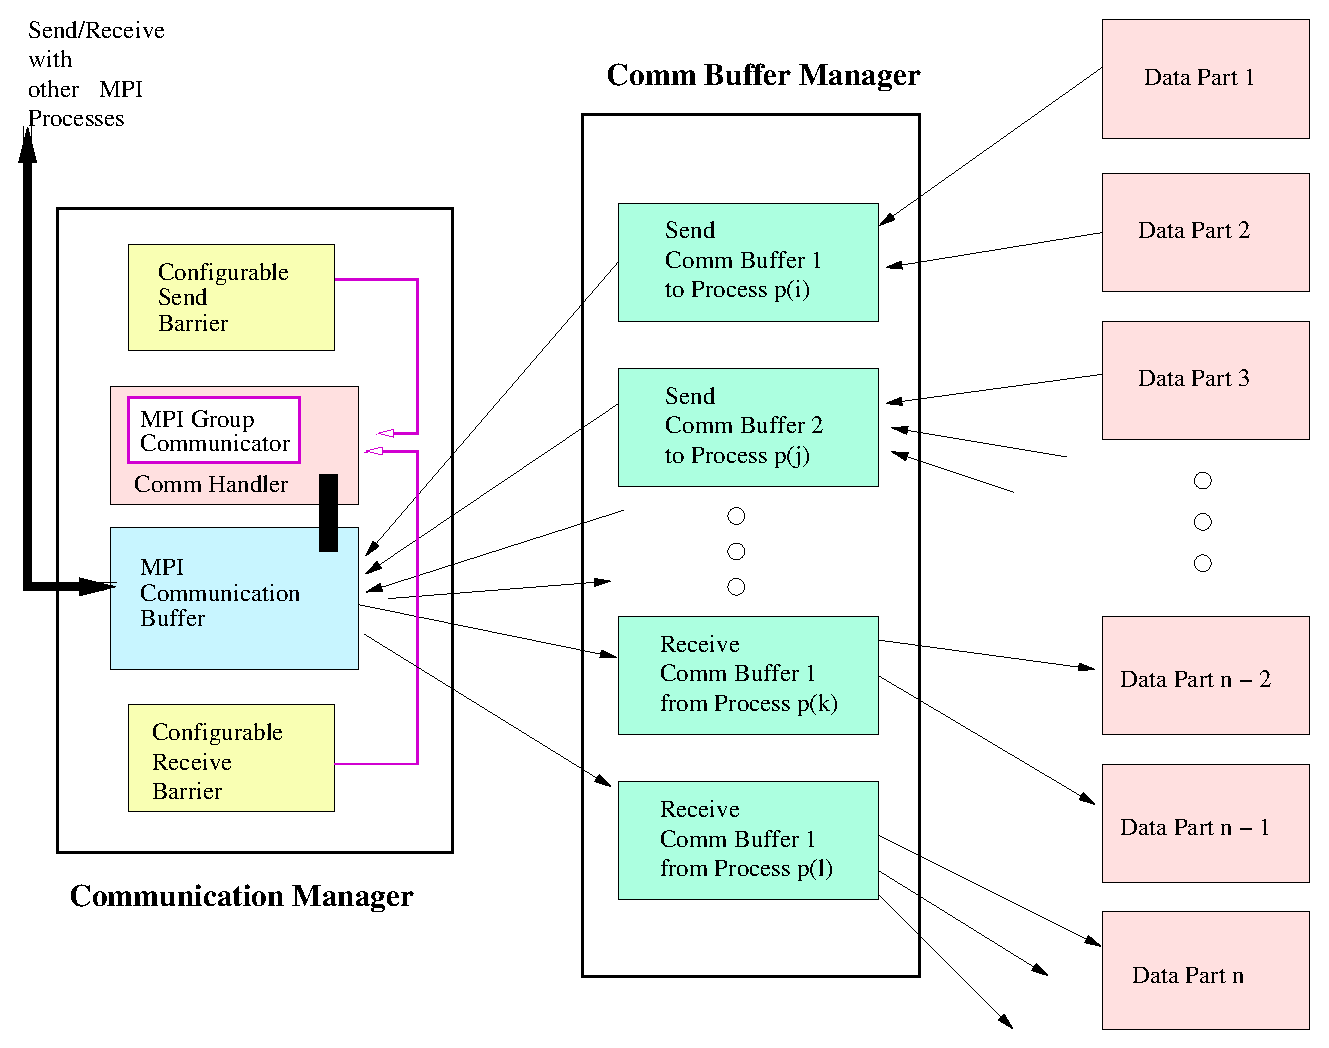
\includegraphics[width=\columnwidth]{Figures/compilation/array-communicator-architecture.eps}
	\caption{The general architecture of a HighP5 communicator responsible for communicating array parts.}
	\label{fig:array-communicator}
\end{figure}

Inside an array communicator, a communication buffer manager component holds one communicator buffer that collects/distributes all elements from a single receiver/sender MPI process from/to various data parts of the current MPI process. Any reordering of array indices in the data parts get unwinded in the communication buffer if it is for sending and is initiated from the buffer if it is for receiving. The various communication buffers feed data to a single MPI group communication buffer if MPI group communication is feasible for the dependency. Data is directly pulled from the communication buffers for point-to-point MPI communications. As there are, possibly, multiple composite PPU controller threads inside an MPI process; the communication manager has configurable parallel barriers inside it separately for send and receive. As a PPU controller thread reaches the point in the flow execution where it is ready to send data, it waits on the send barrier. When all relevent threads reach the barrier, they collaboratively pull content from data parts to communication buffers then from there to the MPI group buffer (if applicable). Finally, the MPI communication is issued by a single thread in the group. For a receive, the sequence of activities is just reversed. If a single confinement of communication dependency does not span all MPI processes then seperate MPI group communicators are initialized for processes of different confinement groups. The barriers are configurable as they allow skipping and merging of steps (often short circuiting send-and-receive) at task launcher initialization at runtime. Similarly, there are alternative implementations of communication buffers that are ideal for different scenarios that the RTE initializer chooses from. Thus, the back-end compiler generates functions for communicator inialization that takes runtime environment information into account for fine-tuning each communicator part.

Except for an all-to-all broadcast scenario, array communicators always use asynchronous versions of MPI communication primitives to maximize computation/communication overlap between and within sender and receiver processes. The send is issued in the earliest LPS transition after the computation stage invocation that updates the underlying array of interest. Meanwhile, the receive is issued in the latest LPS transition before the first computation stage invocation that requires the update. Line 12 to 30 of Listing \ref{luf-comm} shows the invocation of communicator for successive `generatePivotColumn' and `updateUColsBlock' of Listing \ref{highp5-luf}.  
\input{Programs/c-code/block_lu_comm.cc}
If a particular PPU controller thread has no LPU to process for the sender-side stage computation, it still invokes the communicator but with a flag saying that it is `PASSIVE\_REPORTING.' This scenario occurs when the number of LPUs are less than the number of PPUs assigned for a particular LPS-PPS mapping. Invoking the communicator is still needed to ensure correct behavior of the send barrier. In both exceptional and regular scenarios a counter is sent as the second parameter to the communicator. This serves two purposes. First, the counter relates asynchronous receives with sends of a particular iteration of communication. Second, if it is found that the same MPI processes are involved in both send and receive then asynchronous receives are issued early during sending data. Then, the later invocation of `communicator->receive' (as in Line 27) can skip several steps of data reception processing. 

It is critical to use MPI group communications whenever possible when a single MPI process has data to send/receive to/form many MPI processes. In fact, scalability issues with such communications is so wellknown \citep{6312198} that a separate routing network for group communications is common in supercomputers, which MPI group communication primitives take advantage of. A great advantage of portraying the logic of a HighP5 task as a flow of computation across LPSes is that the relative position of the sender and receiver LPSes in the LPS hierarchy and the nature of distribution of the underlying array parts in them dictate what MPI communication primitive is appropriate. Consequently, the back-end compiler generates different types of communicator based on LPS hierarchy and data distribution analysis. The degree of involvement of the positions of LPSes in the choice of a communicator type is illustrated in Figure \ref{fig:map-conf-to-comm}. 

\begin{figure*}[htb]
	\centering
	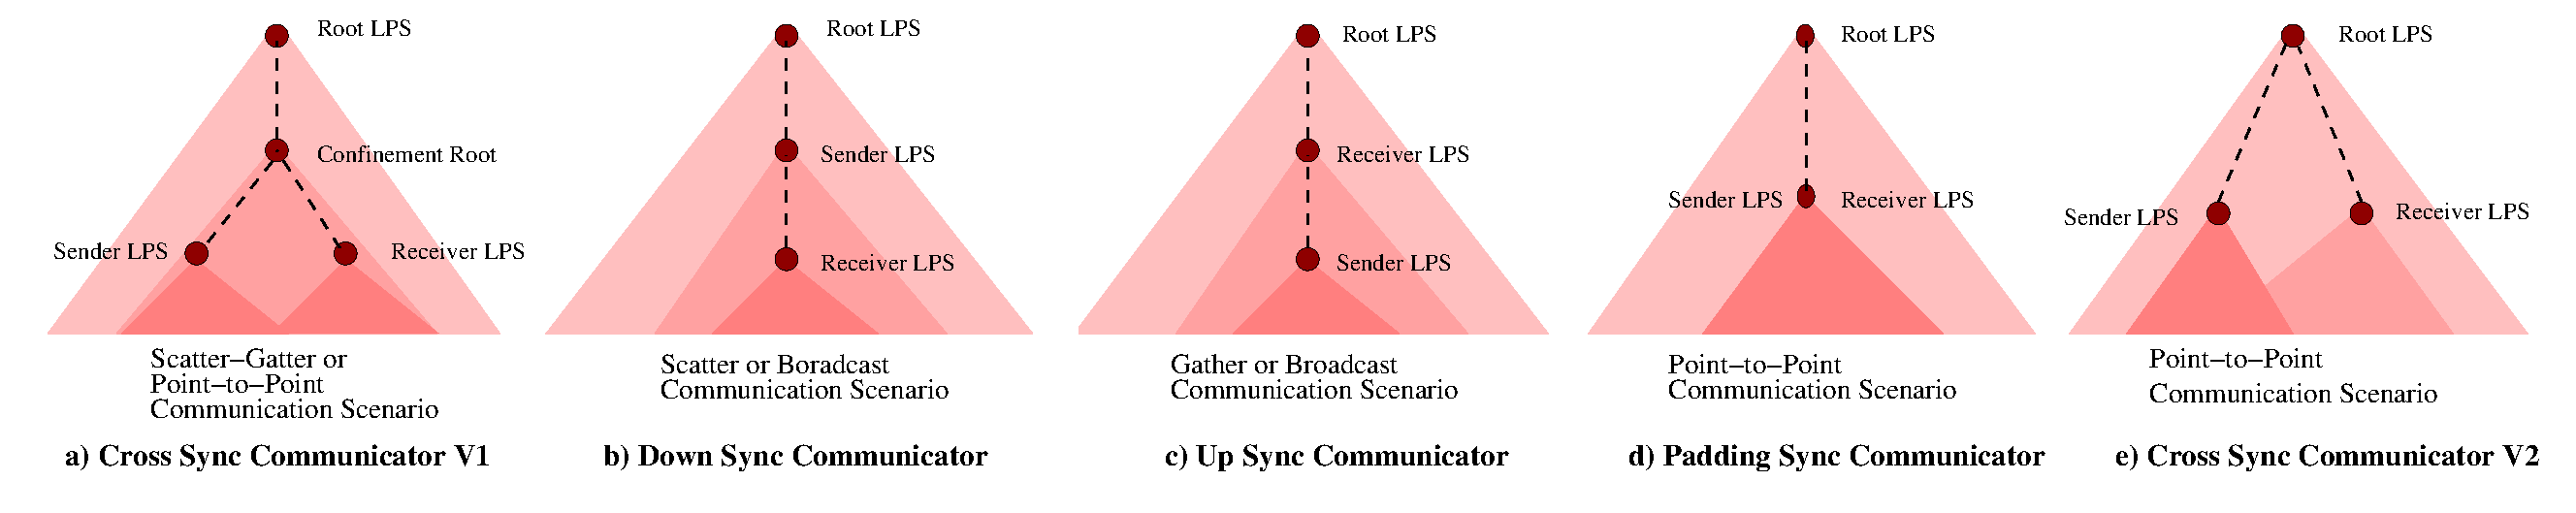
\includegraphics[width=\linewidth]{Figures/compilation/confinement-to-comm-pri.eps}
	\caption{An illustration of how relative positions of the LPSes in the LPS hierarchy involved in a data dependency determine the nature of MPI communication primitives.}
	\label{fig:map-conf-to-comm}
\end{figure*}

The communicator types dictate how data to be exchanged between sender and receiver MPI processes -- not what data to exchange. Given a pair of MPI processes $i$ and $j$, the data $i$ has to send to $j$ for a dependency from LPS1 to LPS2 can be mathematically described as follows:
\begin{equation}
	\begin{split}
		desc(send_{i,j}) = \bigg(\bigcup_{part_{LPS1} \in i}^{}desc(part_{LPS1})\bigg) \\
		\;\cap\;\bigg(\bigcup_{part_{LPS2} \in j}^{}desc(part_{LPS2})\bigg)
	\end{split}
	\label{comm-eq}
\end{equation}
Here, the description of a data part is a multidimensional hierarchical interval function that we discussed in Section \ref{subsec:data-distro}. Given there may be numerous data parts per process, computing intersections on a part-by-part basis is infeasible. To solve this problem, an idea of `part-id-tree folding' is applied on both sender and receiver sides. A folding algorithm recursively generates the most compact interval function description for the data of an LPS in a process of bottom-up contraction of the part-id tree from the interval descriptions of the leaves to the interval description of the root. The approach drastically reduces the number of interval descriptions per process. Subsequently, an interval intersection computation algorithm calculates the interval function for the intersection. These two custom algorithms are part of the common-libraries of RTE that compiler generated code for communication buffers (see Figure \ref{fig:array-communicator}) invokes during their initiation.      

Finally, to determine with what other process to communicate and exactly what data to exchange with a counterpart, an MPI process uses the fact that a PCubeS hierarchy of the execution platform is uniform, and it is possible to get the number of MPI processes using the `MPI\_Comm\_size' function. Aided with the knowledge of confinement roots of each dependency and how that root LPS is mapped to PPSes of the hardware, an MPI process pretends that it has the MPI rank of each candidate other process within its confinement that it may have to exchange data with. This emulation, during a task initialization, of other processes is done with a memory flag that disables allocation of data buffers but keeps intact part-id-tree constructions. Subsequently, the folding algorithm mentioned above is invoked to find compact interval descriptions of all interesting LPU data of that other process and is used for intersection computations with the current process. Therefore, each MPI process finds out what data it needs to exchange with everyone else for each communication dependency without any overhead communication. However, this strategy consumes time. 

\section{Environment Management}
\label{sec:env-mgmt}
Programmers launch the various tasks of a multi-task HighP5 program from a coordinator module/function (called the `Program' in HighP5 terminology). As we stated earlier, the tasks are related to each other by their environment dependencies. To illustrate this concept, we deviate from our running example of block-LU factorization program and present the coordinator module of a multi-task HighP5 conjugate gradient program in Listing \ref{highp5-cg}. Here the solution of a sparse system of equations is computed using iterative interactions among a vector dot-product, vector addition, and sparse matrix-vector multiplication tasks (the coordinator module's logic for this program is easy to understand from the comments embedded in the code). The back-end compiler generates the same intermediate code (equivalent of a main function) for all MPI processes with the decision-making logic embedded in places for the processes to participate in or skip a particular task launch based on their MPI rank and task mapping configuration.   
\input{Programs/Conjugate-Gradient.p}
To implement the concept of successive task executions modifying portions of the environment and there is no accumulation of the results during tasks transitions, the front-end compiler converts the program coordinator module into a flow specification just like the Computation section of a task, then it does a cross-task dependency analysis to setup the data dependency arcs among them. For the back-end compiler, every inter-task data dependency is a potential communication requirement. However, a communicator setup to resolve a data dependency between two tasks is more involved than doing so for an LPS transition within a single task. The reasons for the additional complexity are two. First, it is difficult to compare the data distributions of two tasks using the same data since their LPS hierarchies and LPS-PPS mapping configurations are unrelated. Second, several other task launches may happen between the data updater task and the later task requiring the update, which delays the dependency processing.

The strategy in this regard is to move all task-global data structures under the supervision of environment manager component of the RTE (see Figure \ref{fig:runtime}). External input-outputs (e.g., Lines 12-14 and Line 69 of Listing \ref{highp5-cg}), updates sharing between tasks (e.g., Line 30 and 35), and data generation within a task (e.g., `mvmEnv1.w' of Line 30) for such data structures are all registered as environment instructions in the intermediate C++ code. The back-end compiler generates garbage collection instructions for any task-global data structures that are not needed by any subsequent task executions or external output. These instructions are executed by the task executor during a task initiation and termination based on the instruction type. Consequently, only useful data remain in the collective memory of the MPI processes and unnecessary data are cleaned up. This is even true for multiple versions of the same data within a single task which are generated when the task uses different index-reordering distributions for the data in various LPSes. In that case, the buffers corresponding to the stale versions are reclaimed, keeping the last updated one intact. In addition to the buffers, the interval configuration corresponding to the hierarchical distribution is also retained. The environment manager keeps track of each such data structure using a unique environment linking key.

When a later task needs a data structure updated by an earlier task, it searches the environment manager with the same environment linking key against a data transfer type environment instruction where it supplies its data distribution requirement. The environment manager then compares the stored version's distribution with the distribution asked for and does MPI scatter-gather communications to re-distribute the data, if needed. If the two distributions are equivalent, then no communication occurs and the stored buffer is shared with the new task. If the comparison result dictates that an internal reorganization is sufficient, then again no communication is involved, rather a new version is created for the data within relevant MPI processes.

The current strategy for cross-task data dependency resolution works. However, there are improvement opportunities, such as, avoiding some recurrent computations when the updater and dependent tasks occur within loops and doing the dependency resolution asynchronously and early enough to reduce parallelism opportunity loss during task transitions. We need more sophisticated static analysis in the front-end compiler and rethink the architecture of environment manager and task executors to pursue those improvements.   

\section{Experiments and Analysis}
\label{sec:experience}
To evaluate the efficiency of HighP5 distributed memory compiler, we compared the performance of HighP5 executable with optimized handwritten MPI implementations for three building block applications on the Fugaku supercomputer \citep{9492415}\citep{9658212}. We had a `small project' allocation in the machine for both compiler improvement and performance testing, and we were able to scale our experiments up to $100$ compute nodes. Each Fugaku compute node has $48$ Fugitsu A64FX processors arranged in a group of four $12$-core NUMA nodes with $8$ GB HBM2 integrated memory in them, which gives a total $32$ GB memory per compute nodes. The compute nodes are connected with the Tofu-D interconnect, which is a $6$-D torus network with injection bandwidth of $40.8$ GB/s per node. In general, we had a very fast environment in terms of both computation and communication capacities. Fugaku login nodes are, on the other hand, Intel machines. Hence we used the cross-architecture `mpiFCCpx' provided in the environment as the final C++ compiler to generate executable for the Arm architecture from the intel machines. O3 optimization flag was enabled in the cross platform MPI compiler during compilation for both the reference and HighP5 codes.

In particular, we were interested in assessing how HighP5 programs fare against handwritten MPI programs for applications involving heavy communications. Consequently, the three building block problems of Table \ref{tab:problem-char} were chosen that have a good balance between their computation and communication complexities. In addition, the nature of communication dependencies is also quite different in these problem solutions. Block LU factorization requires directional broadcasts (MPI Bcast, Gather, Scatter, and MPI Reduce) communications in each iteration, finite value estimation using Jacobi iterations (which is commonly called \textit{5-point stencil}) involves pair-to-pair communication (MPI Send/Receive) per iteration for overlapping data synchronization, and conjugate gradient requires multiple all-to-all broadcasts (MPI Allgather and Allscatter) for each gradient descent step.

\begin{table*}[tb]
	\caption{Descriptions of the Building-block Applications being Used for Performance Experiments}
	\small
	\centering
	\resizebox{\textwidth}{!}{
		\begin{tabular}{|l|l|l|l|}
			\hline
			\hline
			& \textbf{Description} & \textbf{Time Complexity} & \textbf{Communication Complexity}  \\
			%\hline
			\textbf{Block LU Factorization} 
			& Diagonalization of a $n \times n$ dense matrix 
			& $\mathcal{O}(n^3)$ 
			& $\mathcal{O}(n^2)$ \\
			%\hline
			\textbf{Finite Value Estimation} 
			& Heat propagation estimation on a $n \times m$ plate for $o$ iterations using $p$ processors 
			& $\mathcal{O}(nmo)$ 
			& $\mathcal{O}(mop)$ \\
			%\hline	
			\textbf{Conjugate Gradient} 
			& Solving a sparse system of $n$ equations using $o$ gradient descend iterations  
			& $\mathcal{O}(n^2o)$
			& $no$ \\ 
			\hline \hline
		\end{tabular}
	}
	\label{tab:problem-char}
\end{table*}

As the reference implementations are pure MPI codes, we used multiple MPI processes per node when running them. Although Fugaku compute nodes have 48 cores, we found that the reference MPI implementations' performance do not improve -- rather, they slightly degrade -- if more than 32 cores per node are used. Hence, block LU factorization and 5-point stencil reference programs were run with $32$ MPI processes per node configuration. However, for the conjugate gradient program, the number of processes per node was further reduced to eight. This is because the Fugaku environment has a limit of $30$ GB memory per node for programs and the input sparse matrix of the conjugate gradient is replicated in all processes, causing a memory fault for large inputs if we increased the process count beyond that. Therefore, the PCubeS model of the platform for HighP5 compiler is also adjusted to have the same degrees of parallelism per-node to maintain parity with the reference codes. However, the HighP5 compiler generates MPI+Pthreads hybrid program as discussed in the earlier section where there is one process per node and intra-node parallelism is achieved using Pthreads (we made an exception to this nature by changing the PCubeS model of the platform during conjugate gradient program compilation for a reason that we will explain later). Furthermore, the operating system installed on the compute nodes of Fugaku does not expose the physical core to logical core ID mapping in the \textit{/proc/cpuinfo} file. Neither does it provide information regarding which core groups share what L2 cache segment. These are information that the HighP5 compiler uses for careful pinning of Pthreads to cores that maximizes cache sharing and reduces synchronization costs. Therefore, the HighP5 versions were slightly at disadvantage that could not be overcome. The reference and HighP5 codes for each node configuration were run 10 times. The standard deviations in 10 runs for all programs are insignificant compared to the average execution times.  

Figure \ref{fig:chart-bluf} compares the average execution time of a block-LU factorization HighP5 program with that of the reference MPI implementation as we step-by-step double the number of nodes from $1$ to $64$ for a large input matrix. We observe that as we increase the number of nodes, HighP5 program's performance keeps improving at a higher rate than the reference and eventually the former surpasses the latter. The reason for better scalability in HighP5 program is that its communication overhead grows at a rate significantly slower than that of the reference implementation since the former uses 32-times fewer processes than the latter. The question is why performance is lagging for small number of nodes. Our finding is that thread synchronization cost is very high in Fugaku compute nodes when the number of threads participating in a synchronization is quite high, which is the case for several intra-node data dependencies in the block-LU program. When the growth of communication overhead outweighs the constant slow synchronization cost inside individual nodes, the HighP5 program surpasses the reference in performance.    
\begin{figure}[htb]
	\centering
	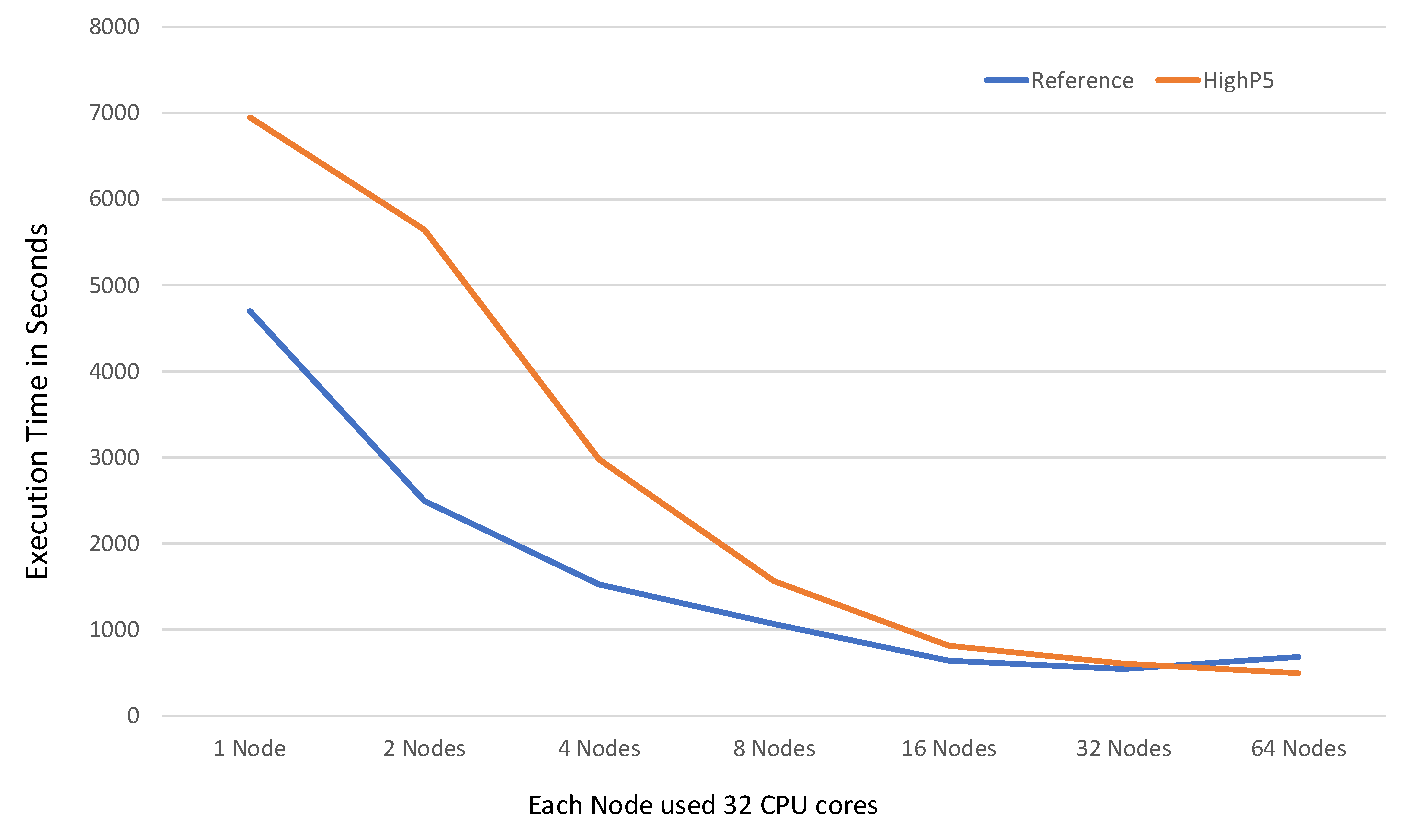
\includegraphics[width=\columnwidth]{Figures/charts/bluf-chart.pdf}
	\caption{Execution time comparison for block LU factorization of a $30720^2$ Square Matrix for different number of nodes.}
	\label{fig:chart-bluf}
\end{figure}

Figure \ref{fig:chart-stencil} demonstrates a reversed trajectory for the average execution times of HighP5 and reference implementations for the 5-point stencil problem. Here, the reference implementation initially lags behind and eventually catches up with the HighP5 implementation. Surprisingly, the reason for this behavior is again the nature  of communication overhead for this program. The stencil algorithm has point-to-point data sharing among processes/threads handling neighboring overlapping partitions. As the number of nodes increases, the computation/communication ratio per thread keeps decreasing, keeping the communication overhead almost fixed due to its point-to-point nature. Consequently, the advantage HighP5 implementation has due to doing more computation per-process keeps decreasing for the fixed input size and eventually both implementations become roughly equivalent. This indicates that for a larger input size, HighP5 implementation should again perform better than the reference for 64 nodes and beyond.    
\begin{figure}[htb]
	\centering
	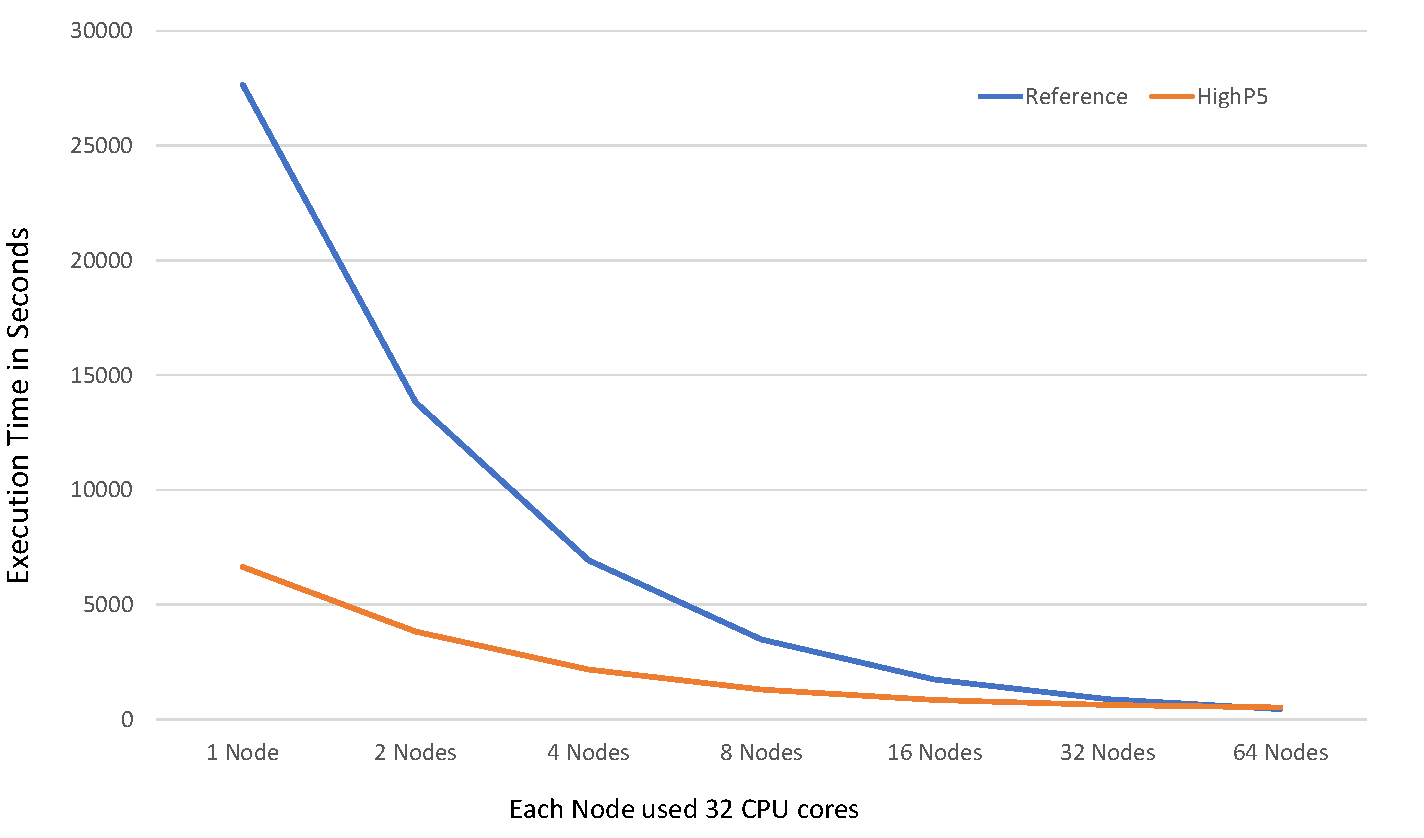
\includegraphics[width=\columnwidth]{Figures/charts/stencil-chart.pdf}
	\caption{Execution time comparison for finite difference calculation on a 204800 by 2048 rectangular plate using hundred thousand Jacobi iterations.}
	\label{fig:chart-stencil}
\end{figure}

An important finding from the first two scalability comparison experiments is that a major obstacle to further performance improvement in HighP5 program is the slowness of group synchronization on the execution platform (in fact, the operating system of the compute nodes). This is a particular concern for our last problem, conjugate gradient, which has three all-thread synchronizations as part of three all-to-all communication per gradient descent iterations. Therefore, we adjusted the PCubeS model of the platform so that the HighP5 compilers generate pure MPI codes for this problem (this adjustment requires a simple property update in the PCubeS model of the hardware). We observe that with this change, the average execution times of the HighP5 implementation are hardly discernible from that of the reference implementation for the conjugate gradient problem for all degrees of parallelism.     
\begin{figure}[htb]
	\centering
	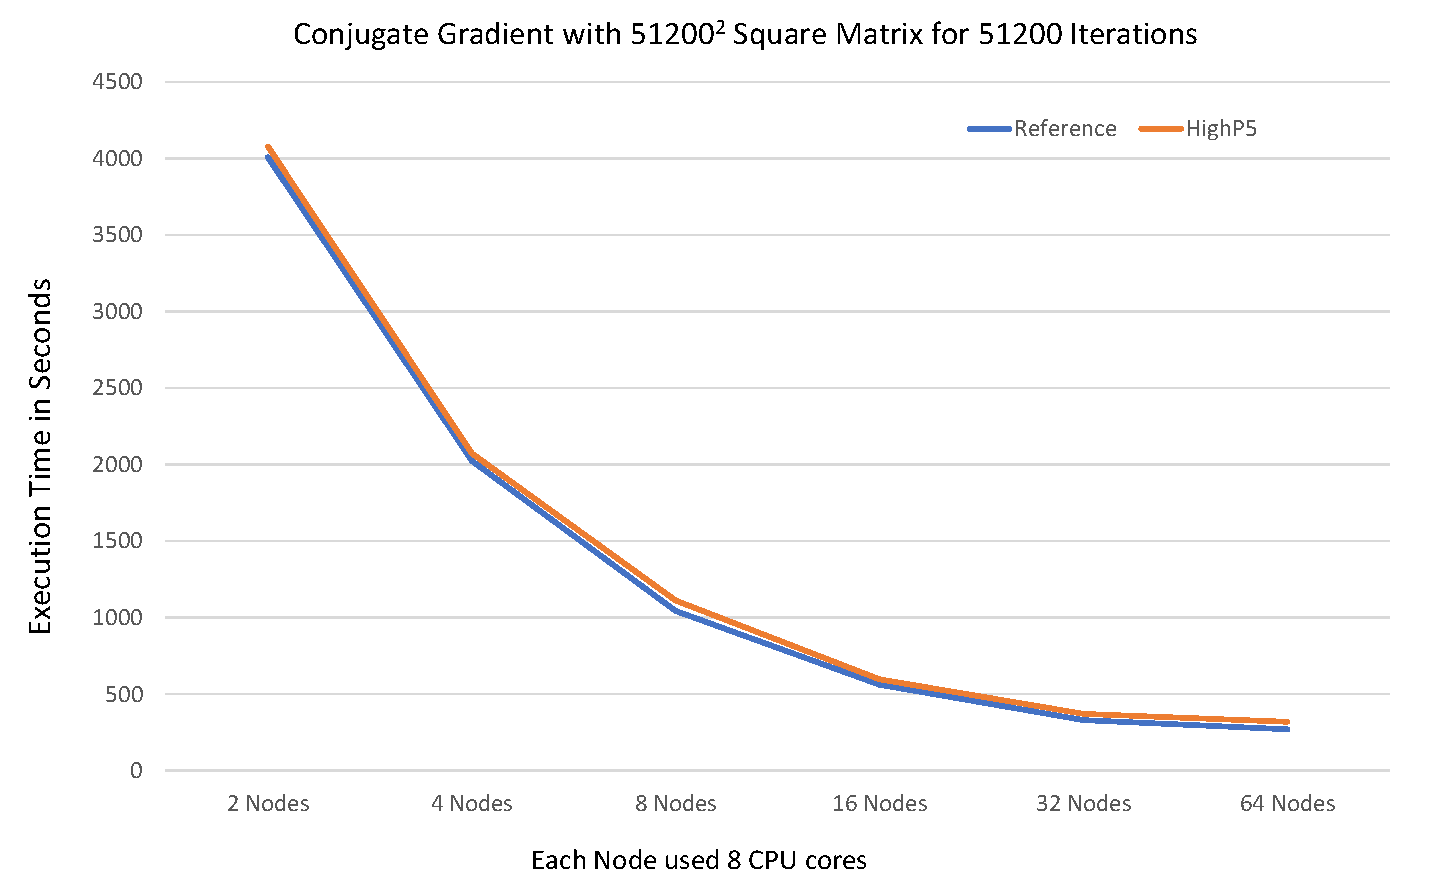
\includegraphics[width=\columnwidth]{Figures/charts/conj-grad-chart.pdf}
	\caption{Execution time comparison for conjugate gradient computation for a 95\% sparse $51200^2$ square matrix for 51200 iterations.}
	\label{fig:chart-cg}
\end{figure}

From the discussions of the previous sections, it is apparent that the intermediate C++ code that the back-end part of the HighP5 compiler emits is significantly more complicated than the reference implementations of the three problems that have problem-specific optimizations related to MPI communication and buffer management. To better understand how different aspects of the generated code affect the overall running time of the executable, we ran HighP5 and reference implementations using 100 nodes and time-logging enabled for larger input sizes for the three building block problems. The input size is chosen in a manner to ensure that each program takes a minimum of $5$ minutes to complete so that meaningful measurements can be taken. Figure \ref{fig:chart-comparison} compares the HighP5 version's decomposition of average execution time with that of the reference where the execution times of reference implementations have been normalized to $1$. In the charts, memory management time refers to the time taken by input/output and all other data structures setup, and communication time includes both the intra-node synchronization and inter/intra-node data movement cost.   
\begin{figure}[htb]
	\centering
	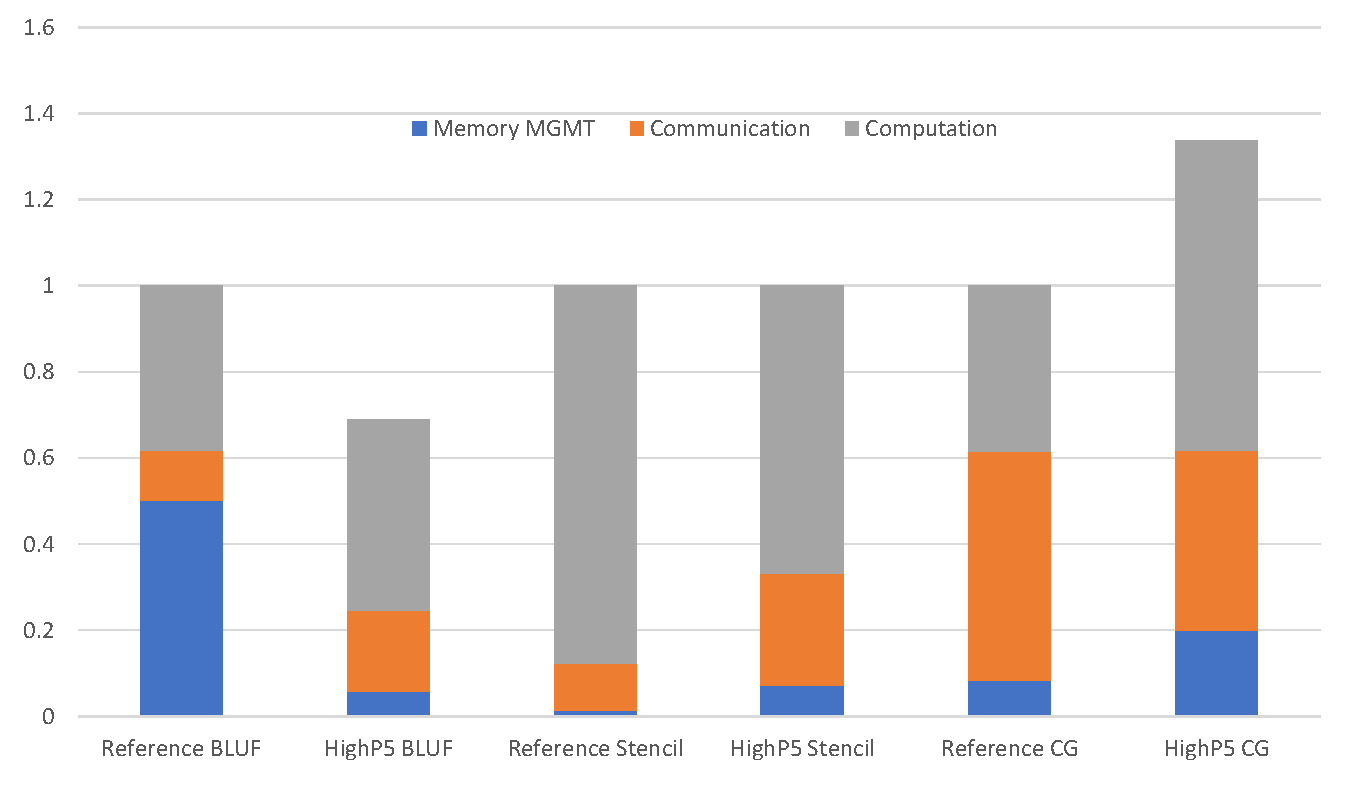
\includegraphics[width=\columnwidth]{Figures/charts/comparison-chart.pdf}
	\caption{Detail breakdown of the normalized execution times for three building block programs with large input sizes and 100 nodes scenario.}
	\label{fig:chart-comparison}
\end{figure}

We observe that HighP5 block-LU factorization is faster than the reference implementation for the $100$ nodes scenario, and the main contributor to the worsening performance in the reference is the memory management overhead. We found that for $100$ nodes and $32$ MPI processes per node in the reference implementation, concurrent file reading for the input matrix is extremely slow. The HighP5 implementation, on the other hand, uses only $100$ open file handles. Setting up other resources (e.g., communicators, and part-id-trees) is actually costlier in HighP5 than in the reference implementation which only needs some buffer allocations. The communication cost is slightly higher in the HighP5 implementation. There are two reasons behind this. The first reason is the slow intra-node synchronization that we discussed earlier. Second, the reference implementation avoids two broadcast communications for scalar variables by replicating some calculations in each MPI processes. Taking advantage of this kind of optimization opportunities in a generic way requires a sophisticated static analysis in the compiler. Finally, the additional computations due to reordered index transformation is almost unnoticeable in the HighP5 implementation's computation time.     

The reference and HighP5 implementations are still on par for the 100 node scenario for the 5-point stencil program. However, the decomposition of execution times is quite different. The HighP5 implementation again takes more time for memory management compared to the reference due to additional data structure setups. For this problem, I/O operation scaled well for a large number of MPI processes due to the fact that they sequentially read data from consecutive chunks of the file, which was not the case for block-LU factorization. The communication cost in HighP5 implementation is higher than that of the reference, again, due to slow synchronizations. However, a smaller cost of computation offsets the higher communication cost. The only sensible explanation for this is better cache utilization through cross-thread collaboration in the HighP5 implementation that the reference cannot avail.

Finally, the HighP5 implementation for the conjugate gradient is slightly slower than the reference implementation. One reason is the higher memory management overhead, which was expected. However, the other reason, a higher computation cost for this problem is a bit surprising. We suspect that since computation per thread/node in this problem is significantly lower than that of the other problems, the overhead computation has a more dominant impact here. We should attempt further improvements in the code generation strategy for computation stages of HighP5 tasks. Finally, as both reference and HighP5 implementations are pure MPI codes for this problem, no slowness in communication time is observed for this problem. However, we are unclear why the communication is slightly faster in the HighP5 version.   

\section{Conclusion}
\label{sec:conclusion}
In this article, we discussed the overall architecture and various aspects of executable generation of the HighP5 programming language compiler for supercomputers and compute clusters that connect multicore/multiprocessor CPU nodes through fast interconnection networks, commonly known as distributed memory machines. As HighP5 uses a unified `PCubeS' architecture abstraction to expose salient features of distributed memory machines, instead of letting programmers directly reason about those features, the compiler has significant additional responsibilities regarding generating efficient binaries from source codes that are not concerns for low-level programming paradigms. The article discusses these responsibilities and their complexities in detail and explains how the HighP5 compiler addresses them. The experimental results on some frequently used building block problems suggest that the compiler is largely successful in generating binaries that are competitive with efficient handwritten, low-level alternatives. However, there are opportunities and challenges associated with further improvements. The explanations and analyses presented in the article should help practitioners and enthusiasts of parallel computing languages and tools development.

As the next step of our research as compiler and language designers, we want to enhance HighP5 programming language with the capabilities of dynamic parallelism that is needed to support problems that occur in fluid-dynamics and astrophysics. Then we will look at the scope of improving the distributed memory compiler further to ensure that updated strategies for executable generation benefit most important programming patterns. There is another HighP5 compiler at its primitive stage that generates binaries for hybrid environments that have both GPUs and CPUs in supercomputer/cluster nodes. However, optimizing the distributed memory compiler to the extent possible is more urgent as the compiler for hybrid environments needs to answer the same questions regarding CPU host usage and cross-node communication optimization. It just has additional responsibilities regarding efficient utilization of the GPUs.    


%\backmatter
\bmsubsection*{Author Contributions}
Muhammad Nur Yanhaona is the primary contributor of this research work. He worked under the supervision of Andrew Grimshaw.

\bmsubsection*{Acknowledgments}
We thank Shahriar Hasan Mickey, who served as a voluntary research assistant of Muhammad Nur Yanhaona during the beginning phases of the project and helped with setting up the experimental environment. We also thank Riken Institute of Japan for providing us with access to the Fugaku supercomputer which was critical for compiler improvement activities and experiments conduction. 

\bmsubsection*{Financial Disclosure}
None reported.

\bmsubsection*{Conflicts of Interest}
The authors declare no conflicts of interest.

\bmsubsection*{Supporting Information}
The source code of the compiler, HighP5 and reference source codes used for experiments, and the detail of performance results reported in this paper are all available in the Fugaku branch of the Github repository \href{https://github.com/yanhaona/HighP5-Updated.git}{HighP5-Compilers}.

\bibliographystyle{wileyNJD-Chicago}
\bibliography{refs}


\end{document}
